%%
%% This is file `sample-acmsmall.tex',
%% generated with the docstrip utility.
%%
%% The original source files were:
%%
%% samples.dtx  (with options: `acmsmall')
%% 
%% IMPORTANT NOTICE:
%% 
%% For the copyright see the source file.
%% 
%% Any modified versions of this file must be renamed
%% with new filenames distinct from sample-acmsmall.tex.
%% 
%% For distribution of the original source see the terms
%% for copying and modification in the file samples.dtx.
%% 
%% This generated file may be distributed as long as the
%% original source files, as listed above, are part of the
%% same distribution. (The sources need not necessarily be
%% in the same archive or directory.)
%%
%% Commands for TeXCount
%TC:macro \cite [option:text,text]
%TC:macro \citep [option:text,text]
%TC:macro \citet [option:text,text]
%TC:envir table 0 1
%TC:envir table* 0 1
%TC:envir tabular [ignore] word
%TC:envir displaymath 0 word
%TC:envir math 0 word
%TC:envir comment 0 0
%%
%%
%% The first command in your LaTeX source must be the \documentclass command.
\documentclass[acmsmall,review,screen]{acmart}
%% NOTE that a single column version is required for 
%% submission and peer review. This can be done by changing
%% the \doucmentclass[...]{acmart} in this template to 
%% \documentclass[manuscript,screen]{acmart}
%% 
%% To ensure 100% compatibility, please check the white list of
%% approved LaTeX packages to be used with the Master Article Template at
%% https://www.acm.org/publications/taps/whitelist-of-latex-packages 
%% before creating your document. The white list page provides 
%% information on how to submit additional LaTeX packages for 
%% review and adoption.
%% Fonts used in the template cannot be substituted; margin 
%% adjustments are not allowed.
%%
%% \BibTeX command to typeset BibTeX logo in the docs
\AtBeginDocument{%
  \providecommand\BibTeX{{%
    \normalfont B\kern-0.5em{\scshape i\kern-0.25em b}\kern-0.8em\TeX}}}

%% Rights management information.  This information is sent to you
%% when you complete the rights form.  These commands have SAMPLE
%% values in them; it is your responsibility as an author to replace
%% the commands and values with those provided to you when you
%% complete the rights form.
%\setcopyright{acmcopyright}
%\copyrightyear{2022}
%\acmYear{2022}
%\acmDOI{XXXXXXX.XXXXXXX}


%%
%% These commands are for a JOURNAL article.
%\acmJournal{PACMPL}
%\acmVolume{0}
%\acmNumber{0}
%\acmArticle{166}
%\acmMonth{0}

%%
%% Submission ID.
%% Use this when submitting an article to a sponsored event. You'll
%% receive a unique submission ID from the organizers
%% of the event, and this ID should be used as the parameter to this command.
\acmSubmissionID{166}

%%
%% For managing citations, it is recommended to use bibliography
%% files in BibTeX format.
%%
%% You can then either use BibTeX with the ACM-Reference-Format style,
%% or BibLaTeX with the acmnumeric or acmauthoryear sytles, that include
%% support for advanced citation of software artefact from the
%% biblatex-software package, also separately available on CTAN.
%%
%% Look at the sample-*-biblatex.tex files for templates showcasing
%% the biblatex styles.
%%

%%
%% The majority of ACM publications use numbered citations and
%% references.  The command \citestyle{authoryear} switches to the
%% "author year" style.
%%
%% If you are preparing content for an event
%% sponsored by ACM SIGGRAPH, you must use the "author year" style of
%% citations and references.
%% Uncommenting
%% the next command will enable that style.
%%\citestyle{acmauthoryear}
\usepackage{float}
\usepackage{fancyvrb}
\usepackage{enumitem}
%%
%% end of the preamble, start of the body of the document source.
\begin{document}

%%
%% The "title" command has an optional parameter,
%% allowing the author to define a "short title" to be used in page headers.
\title{ZKSNARK WASM Emulator}

%%
%% The "author" command and its associated commands are used to define
%% the authors and their affiliations.
%% Of note is the shared affiliation of the first two authors, and the
%% "authornote" and "authornotemark" commands
%% used to denote shared contribution to the research.
%\author{Sinka Gao}
%\authornote{All authors contributed equally to this research.}
%\email{xgao@zoyoe.com}
%\orcid{1234-5678-9012}
%\author{Hongfei Fu}
%\email{jt002845@sjtu.edu.cn}
%\author{Heng Zhang}
%\email{shindar90@gmail.com}
%\author{Junyu Zhang}
%\email{junyu92@gmail.com}
%\author{Guoqiang Li}
%\email{li.g@sjtu.edu.cn}
%\orcid{0000-0001-9005-7112}


%\authornotemark[1]
%\affiliation{%
%  \institution{Delphinus Lab.}
%  \streetaddress{P.O. Box 1212}
%  \city{Sydney}
%  \state{NSW}
%  \country{Australia}
%  \postcode{43017-6221}
%}

%\authornotemark[2]
%\affiliation{%
%  \institution{Shanghai Jiao Tong University}
%  \streetaddress{800 Dongchuan Rd.}
%  \city{Shanghai}
%  \country{China}
%  \postcode{200240}
%}

%%
%% By default, the full list of authors will be used in the page
%% headers. Often, this list is too long, and will overlap
%% other information printed in the page headers. This command allows
%% the author to define a more concise list
%% of authors' names for this purpose.
%\renewcommand{\shortauthors}{Sinka and Li, et al.}


%% commands
\newcommand{\zkwasm}{ZKWASM}
\newcommand{\zksnark}{ZKSNARK}
\newcommand{\initstate}{$(\mathbf{I}(\mathbf{C},\mathbf{H}), \mathbf{E}, \mathbf{IO})$}
\newcommand{\fullstate}{$(iaddr, \mathcal{F}, \mathcal{M}, \mathcal{G}, \mathcal{SP}, \mathbf{I}, \mathbf{IO})$}
\newcommand{\partialstate}[2]{$(\mathcal{F}, \mathcal{M}_{[#1,#2]}, \mathcal{SP}_{[#1,#2]}, \mathbf{I}(\mathcal{C,\mathcal{H}}), \mathbf{IO})$}
\newtheorem{remark}{Remark}
%%
%% The abstract is a short summary of the work to be presented in the
%% article.
\begin{abstract}
WebAssembly, or WASM for short, is a binary code format for a stack-based virtual machine, first published in 2018 and now becomes a main-steam technology for providing distributed serverless functions.
  %In just several short years, it established a solid ecosystem from complex distributed applications to serverless functions served on large cloud infrastructure providers like Azure and AWS Lambda.
Recently, the demand for privacy and trustless serverless functions has started to grow in cloud, edge, and grid computation, which poses a question for those serverless function providers: what feature they need to add to make WASM runtime more secure so that the application run on top it become trustless to their users.
To address this, we leverage the technology \zksnark\,  (zero-knowledge Succinct Non-interactive Argument of Knowledge),  a powerful proof system that allows efficient verification of the evaluation problem of statements, to give WASM runtime the ability to provide trustless computation service. More precisely, we present \zkwasm, a \zksnark\, backed virtual machine that emulates the execution of WASM bytecode and generates zero-knowledge-proofs for the emulation result. The proof generated by the \zkwasm\, virtual machine can then be used to convince an entity, with no leakage of confidential information, that the result of the emulation enforces the semantic specification of WASM. 
\end{abstract}

%%
%% The code below is generated by the tool at http://dl.acm.org/ccs.cfm.
%% Please copy and paste the code instead of the example below.
%%
\begin{CCSXML}
<ccs2012>
 <concept>
  <concept_id>10010520.10010553.10010562</concept_id>
  <concept_desc>Computer systems organization~Embedded systems</concept_desc>
  <concept_significance>500</concept_significance>
 </concept>
 <concept>
  <concept_id>10010520.10010575.10010755</concept_id>
  <concept_desc>Computer systems organization~Redundancy</concept_desc>
  <concept_significance>300</concept_significance>
 </concept>
 <concept>
  <concept_id>10010520.10010553.10010554</concept_id>
  <concept_desc>Computer systems organization~Robotics</concept_desc>
  <concept_significance>100</concept_significance>
 </concept>
 <concept>
  <concept_id>10003033.10003083.10003095</concept_id>
  <concept_desc>Networks~Network reliability</concept_desc>
  <concept_significance>100</concept_significance>
 </concept>
</ccs2012>
\end{CCSXML}

%\ccsdesc[500]{Computer systems organization~Embedded systems}
%\ccsdesc[300]{Computer systems organization~Redundancy}
%\ccsdesc{Computer systems organization~Robotics}
%\ccsdesc[100]{Networks~Network reliability}

%%
%% Keywords. The author(s) should pick words that accurately describe
%% the work being presented. Separate the keywords with commas.
%\keywords{datasets, neural networks, gaze detection, text tagging}

\received{10 November 2022}
%\received[revised]{12 March 2009}
%\received[accepted]{5 June 2009}


%%
%% This command processes the author and affiliation and title
%% information and builds the first part of the formatted document.
\maketitle

\section{Introduction}
WASM (or WebAssembly), is an open standard binary code format close to assembly. Its initial objective is to provide an alternative to java-script and better performance in the current web ecosystems. Benefit from its platform independence, front-end flexibility (can be compiled from the majority languages including C, C++, assembly script, rust, etc.), good isolated run-time and speed that close to native binary, its usage start to arise in distributed cloud and edge computing. Recently it becomes a popular binary format for users to running customized functions on AWS Lambda, Open Yurt, AZURE, etc.

As with the technology of WASM run-time for cloud and edge computing shifts, security and privacy \cite{ pearson2009taking} issues emerge in scenarios that demanding trustless \cite{wood2016trustless, chang2002trustless} computation and privacy computing \cite{xiao2012security,takabi2010security}. For instance, suppose that there is a voting hub  hosted in the cloud to collect votes for proposals. The role of this service is to reporting voting result to users while does not leaking any information of any voter's choice. In this scenario, we would like the service does not only provide the voting result but also provide a proof to convince users that the provided result is calculated with predefined protocols (voting protocols). However since the service can not leak voters' personal choice, they should not reveal any voting ticket that is signed by a voter which makes it tricky to make a proof. 

Traditional ways to achieve trustless and privacy usually involves invasive changes to the source code of the service running on cloud and those changes are usually applied in a case by case manner. In this work, instead of change the code itself, we propose a novel approach by implementing \zkwasm, which is a WASM virtualy machine that does not only runs the WASM bytecode but also provides a zero-knowledge proof which is used to convince a verifier that the execution result is trustworthy.

The idea of \zkwasm\, is derived from ZKSNARK (Zero-Knowledge Succinct Non-Interactive Argument of Knowledge) which is a combination of SNARG (Succinct non-interactive arguments) and zero-knowledge proof. In general, adoption of ZKSNARK usually requires implementing program in arithmetic circuits (see Section \ref{chp:arith-circuits}) which forms a barrier for existing programs to leverage the power of it. Thus in this paper, we writes the whole WASM virtual machine in ZKSNARK circuits so that existing WASM applications can benifit from ZKSNARK by simply running on the \zkwasm\, without any modification. Therefore, the cloud service provider can prove to any user that the computation result is computed honestly and no privacy information is leaked.

\smallskip\noindent\textbf{The Problem.}
To implement a ZKSNARK backed WASM virtual machine, we need to connect the implementation of WASM runtime with the prove system of ZKSNARK. In general, a ZKSNARK system is represented in arithmetic circuits (see Section \ref{chp:arith-circuits}) with polynomial constraints. Therefore we need to abstract the full imperative logic of a WASM virtual machine systematically and rewrite it into arithmetic circuits with constraints. Given two outputs, one is generated by emulating the WASM bytecode in WASM runtime that enforce the semantic of WASM specification, and the other satisfies the constraints imposed on the arithemtic circuits, if the circuits we write preserves the semantic, then these two ouputs must be same. Thus the proof of the ZKSNARKS derived from the circuits also shows that the output is valid as a result of emulating the bytecode in WASM runtime. 

\smallskip\noindent\textbf{Our Contribution.}
In this paper we systematically abstract the WASM runtime implementaion and rewrite it into arithmetic circuits with constraints. By doing so, we proposed and implemented the first zk-WASM virtual machine that supports web assembly specification. Moreover, by providing \zkwasm\, existing program compiled to WASM (without any modification) can then satisfy the privacy and trustless requirements that recently emerges in cloud and edge computing.

\smallskip\noindent\textbf{Organization of the Paper.}
After a brief introduction about the basic ideas about how to connect statefull virtual machine with SNARK in Section \ref{chp:preliminary}, we describe the basic building block and ingredients use used to construct \zkwasm circuits in Section \ref{chp:constraint-system} and then presents the circuits architecture in Section \ref{chp:architecture-circuits}. After the architecture is fixed, we list circuit of each opcode of WASM in Section \ref{chp:instruction-circuits}. In Section \ref{chp:foreign} we discuss foreign instruction expansion which provides a way to extend the virtual machine for better performance and integration. In the end, we discuss the performance benchmark in Section \ref{chp:performance}.

\section{Preliminaries}
\label{chp:preliminary}
\subsection{Succinct Verification}
Succinct non-interactive arguments (SNARGs) enable verifying NP statements with lower complexity than required for classical NP verification. Traditionally, the focus has been on minimizing the length of such arguments; nowadays researches have focused also on minimizing verification time, by drawing motivation from the problem of delegating computation.

Recent constructions of preprocessing SNARGs have achieved attractive features: they are publicly-verifiable, proofs consist of only O(1) encrypted (or encoded) field elements, and verification is via arithmetic circuits of size linear in the NP statement. Additionally, these constructions seem to have “escaped the hegemony” of probabilistically-checkable proofs (PCPs) as a basic building block of succinct arguments.


\subsection{Polynomial Commitment Schemes}
PCS (Polynomial Commitment Schemes \cite{boneh2020halo-pcs,boneh2020efficient-pcs,kate2010polynomial-pcs}) is a powerful tool to construct SNARK schemes for the statement of polynomial evaluation. PCS provides a way for prover and verifier to commit to a polynomial $p$ and then open the commitment at certain any point (prove that the evaluation of $P$ a point $x$ is equal to a claimed value $v$). In this paper, if without specification, We use KZG (Kate, Zaverucha and Goldberg) as our polynomial commitment scheme and the commitment formula for a polynomial $p$ is defined by $g^{p(\beta)}$ where $\beta$ is a random value negioated by prover and verifier at setup stage and $g$ is a point on a special elliptic curve.

\subsection{Stateless Programs as Arithmetic Circuits}
\label{chp:arith-circuits}
Once there exists a SNARK scheme for a prover to prove the evaluation of polynomials $p_i$ at $x_i$ to a verifier, we can then construct SNARK for a prover to prove that a program $P(X)$ has certain return value $v$ when input $X$ is provided. Many such construction can be found in literature such as Groth, Sonic, Marlin, Plonk, etc. In this paper, we construct our ZK virtual machine using the proof system of Halo2, which is an extension of PLONK (See Section \ref{chp:constraint-system}). In PLONK setup, stateless programs can be encoded into a special format called arithmetic circuits.

An arithmetic circuit is a set of gates and each gates can have a set of inputs that need to be processed and a set of outputs that can be used as other gates' inputs. The gates can be connected together so as to carry out an arithmetic algorithm. In the end, the outputs of the circuit is result of the algorithm. For example, suppose that we need to represent an sum algorithm can be constructed by a list of add gates as in Figure \ref{fig:sum-gates}.

\begin{figure}[!ht]
\centerline{
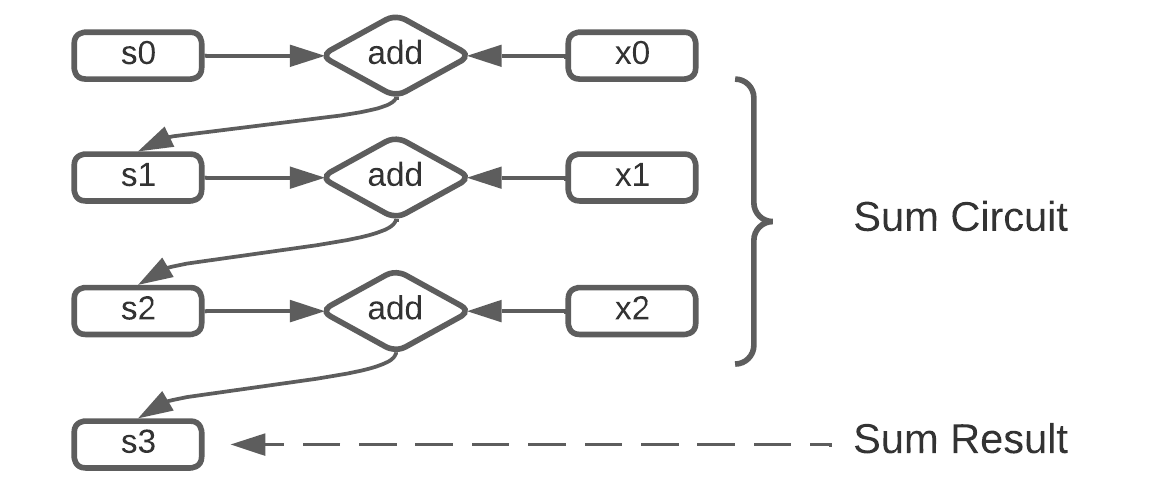
\includegraphics[scale=0.8]{figs/arithment-circuit.png}
}
\caption{Arithment Circuit of Sum}\label{fig:sum-gates}
\end{figure}

Now we have connected stateless programs to arithmetic circuits, and we know how to construct SNARKS of polynomial evaluation using PCS. Therefore it remains to establish a connection between arithmetic circuits with polynomials. This can be achieved by using interpolation techniques and copy constraints in PLONKish (see Section \ref{chp:constraint-system}).

%PCS 是polynomialbase的,constraint base ---> PCS
\subsection{Connecting Stateful Virtual Machine with Arithmetic Circuits}
\label{chp:encode-state-in-circuits}
Now we need to make a setup further, instead of construct a SNARK scheme for stateless programs, we would like to construct a SNARK scheme for a stateful virtual machine. We do not constructing such SNARK from scratch, we construct it from the knowing ingredients which are the arithmetic circuits in Section \ref{chp:arith-circuits}. 

To start with, we establish the connection between a virtual machine and a program by treating the virtual machine as a program which generates a list of state transitions and each transition is defined as a monad function between states. We denote the transition function as $T_i$ which takes an input $s:State$ and outputs a new state $s':S$. The type of state $\mathcal{S}$ is defined as a tuple of \fullstate \, where $\mathcal{F}$ is the calling frame, $\mathcal{M}$ is the memory state, $\mathcal{S}_p$ is stack and $\mathcal{I}$ is the image which contains code image $\mathcal{C}$ and initial memory $\mathcal{H}$.

Also for an instruction $op$ at address $addr$ in the image $\mathcal{I}$ of a WASM binary file, we define the transition semantic of $op$ to be a pair of $(t^{addr}_{op}, c^{addr}_{op})$ where $t^{address}_{op}$ is a state transition function and $c^{addr}_{op}$ is the control flow function from $S$ to the address of next instruction.

To define a valid sequence of transitions $T_i$, we first requires that $T_0$ enforces the transition semantic of the instruction at the entry point $iaddr$ and for all $addr, s, k$, $T_k(s) = t^{iaddr}_{op}(s) \rightarrow T_{k+1} = t_{op'}^{iaddr'}$ where $iaddr' = c_{op}^{iaddr}(s)$ and $op'$ is the opcode of the instruction at $'iaddr$.

Second, with this setup we can mapping execution of a executable image $I$ in a virtual machine $\mathcal{V}_m$ to a sequence of transition function $T_i$ over an initial state $s_0$. By denoting $s_i = T_i (T_{i-1}(\cdots T_0(s_0)))$ and $s_e$ to be the last state of the transition sequence, We require the final opcode of $T_{e}$ is return and the depth of the calling frame of $s_e$ is zero $\mathcal{F}(s_e).depth = 0$.

We say a system of arithmetic circuits $C$ of transitions is equivalent to a WASM virtual machine if for any given entry point $iaddr_0$ there exists a unique sequence of $T_i$ satisfies $C$ and $T_0 = c^{iaddr_0}_{op}$.

%Stateless -> Statefull 的虚拟机:monadic function while s is hash
\subsection{Leverage zero-knowledge in ZKWASM}
A zk-SNARK is a SNARK scheme that provide a way for a prover to prove statements without leaking any information. When we construct the above SNARK scheme for virtual machine in a zero-knowledge way, then we create a ZK Virtual machine that can prove the execution of certain program image without leaking any information.  This feature makes the ZK virtual machine extremely useful in scenarios where the prover would like to prove that certain ouput is calculated from execution a particular program image but does not want to leak the data used.
 

\section{Preliminaries}
\label{chp:preliminary}
Throughout the paper, we use the notation $a:A$ to specify a variable of type $A$,  $\mathbf{F}$ to specify a number field, and $\mathbf{F}^{n}$ to specify a multi-dimensional vector with dimension $n$. We denote  by $A \rightarrow B$ the function type from $A$ to $B$ and use $\circ$ to denote function composition. Moreover, we use $\mathbf{G}[i][j]$ to specify the value of the cell of matrix $\mathbf{G}$ at the $i$th row and $j$th column.

\subsection{WASM Run-Time as a State Machine}
\label{chp:exec-trace}
We consider the WASM virtual machine as a gigantic program, with the input as a tuple \initstate, where $\mathbf{I}$ is a WASM executable image that contains a code image $\mathbf{C}$ and an initial memory $\mathbf{H}$, $\mathbf{E}$ is its entry point, and $\mathbf{IO}$ represents the $(\mathbf{stdin}, \mathbf{stdout})$ firmware. In the serverless setup, the WASM run-time starts with an initial state based on the loaded image $\mathbf{I}$, then jumps to the entry point $\mathbf{E}$ and starts executing the bytecode based on the WASM specification. 

Internally the WASM run-time maintains a state $\mathcal{S}$ denoted by \fullstate \, where $iaddr$ is the current instruction address, $\mathcal{F}$ is the calling frame with a $depth$ field, $\mathcal{M}$ is the memory state, $\mathcal{SP}$ is the stack and $\mathcal{G}$ is the set of global variables. The run-time simulates the semantic of each instruction start at $\mathbf{E}$ until it reaches the exit. The instructions it simulates form an execution trace $\left[t_0, t_1, t_2, t_3, \cdots \right]$ and each transition $t_i$ is a function between states which takes an input $s:\mathcal{S}$ and outputs a new state $s':\mathcal{S}$. For simplicity, we will use the notation of record field to specify a field in state $s:\mathcal{S}$. For example, $s.iaddr$ denotes the current instruction address of state $s$, $s.\mathbf{IO}.\mathbf{stdin}$ denotes the input of state $s$, etc. We also use $op(iaddr)$ to denote the opcode (operation code that specifies the operation to be performed) at address $iaddr$ in the code section $\mathcal{C}$ of image $\mathbf{I}$.

\smallskip Based on the above definition, we define the criteria for a list of state transitions to be valid under \initstate, as follows.

\begin{definition}[Valid Execution Trace]
\label{def:valid-trace}
Given a WASM machine with input \initstate, and $s_0$ is the initial state with $s_0.iaddr = \mathbf{E}$. A valid execution trace is a list of transition functions $t_i$ such that the following holds:
\begin{enumerate}[leftmargin=*]
\item $t_0$ matchs the semantic of the instruction $op$ at the entry $iaddr_0 = \mathbf{E}$.
\item For all $k$, $s_k = t_{k-1} \circ \cdots t_1 \circ t_0 (s_0)$, $t_k$ enforces the semantics of $op(s_k.iaddr)$.
\item If $s_{e}$ is the last state, then the depth of the calling frame is zero: $s_e.\mathcal{F}.depth = 0$.
\end{enumerate}
\end{definition}

We take the output of the final state $s_e.\mathbf{IO}.output$ to be the result of the WASM run-time with input \initstate. The $output$ is a valid result if and only if there exists an valid execution sequence $\left[t_0, t_1, \cdots \right]$ such that $s_e$ is the last state of $t_i$ under \initstate.

 
\subsection{Succinct Proof of a Program}

Compared with a standard WASM runtime, \zkwasm\, aims to provide a proof to prove that the output is valid so that it can be used in scenarios which require trustless and privacy computation.  Moreover, the verifying algorithm needs to be simple in the sense of complexity to be useful in practical. Before we dive into how to construct such a proving and verifying scheme for the complex WASM run-time, we go through a few basics about how to construct such a scheme for functions.

Suppose that we have a pure function $f$, a list of parameters $params$ for $f$, an entity $A$ that calculates $r = f(params)$ and an entity $B$ that would like to know $r$ but does not willing to do the exact computation. A scheme that enables $A$ to prove to $B$ about the correctness of $r$ is of great interests in cryptography design if the complexity for $B$ to verify the proof is negligible comparing to the complexity to do the actual calculation. If such a scheme is not interactive and the verifying complexity is negligible comparing to the initial complexity of $f$, then we say it is a SNARK (succinct non-interactive argument of knowledge).

\smallskip Topics about constructing SNARK has been well studied in the literature \cite{groth2011efficient, groth2017snarky,groth2016size,groth2017snarky, bootle2016efficient,bunz2018bulletproofs, maller2019sonic, chiesa2020marlin,bunz2020transparent} where functions $f$ are defined by a computational program $\mathbf{P}$.
A common approach for constructing such SNARK is to turn the program $\mathbf{P}:\mathbf{F}^m\rightarrow \mathbf{F}^r$ into a special form of constraint systems $C_i(x) = 0$ (where $C:\mathbf{F}^n \rightarrow \mathbf{F}$), such that for any parameters $param: \mathbf{F}^m$ of $\mathbf{P}$, there exists a unique vector of witness $w:\mathbf{F}^{n-m-r}$ and a unique vector of result $r:\mathbf{F}^r$ that satisfy
\[
C_i(param_0, param_1, \cdots, w_0, w_1, \cdots, r_0, r1, \cdots) = 0.
\]
\noindent We call such constraint system arithmetic circuits (see \ref{chp:arith-circuits} for the precise definition). Once the arithmetic circuits are constructed based on $\mathbf{P}$, the problem of proving $\mathbf{P}(params) = r$ becomes the problems of finding witness vector $w$ and prove that the vector $v = (params;w;r)$ satisfies $C(v) = 0$.
%(see Figure \ref{fig:sum-gates} for an example of constraints on summarize function).
%\begin{figure}[!ht]
%\centerline{
%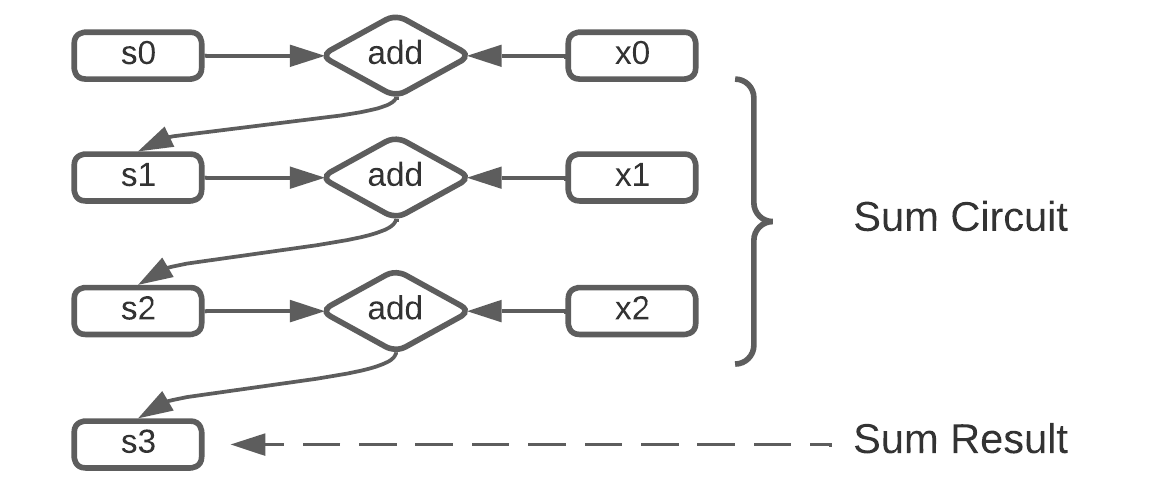
\includegraphics[scale=0.8]{figs/arithment-circuit.png}
%}
%\caption{Arithment Circuit of Sum}\label{fig:sum-gates}
%\end{figure}

\smallskip Thus the problem of constructing SNARK for a program $\mathbf{P}$ is turned into the problem of constructing SNARKS for the constraint system $\mathbf{C}$. Different shapes of $\mathbf{C}$ may have different SNARK construction, and the base idea to construct SNARK for $\mathbf{C}$ is to turn the proof for the constraint system $\mathbf{C}$ into proofs of polynomial evaluations, that is deriving a list of polynomials $p$ and a list of evaluation pairs $(x_i,v_i)$ such that $\forall i, p_i(x_i) = v_i$ implies $\mathbf{C}$. The technical and implementation details of such transform is not the focus of this paper, thus we omit the details and give an example to motivate the basic technique behind it.
%which is compressing the list of multi-linear discrete equations in $\mathbf{C}$ into polynomial equations via interpolation.
For example, suppose that a constraint system $\mathbf{C}_i(x) = 0$ can be rewritten into the matrix form $\sum_j c_{ij}x_j = 0$ (linear constraints are used here for simplicity). Then by Lagrange interpolating on each column vector of $\mathbf{C}$ and vector $x$ we get a list of polynomials $\bar{c}_i(X)$ and $\bar{p}(X)$ such that $\bar{c}_i(j) = c_{ij}$ and $\bar{p}(j) = x_j$. Therefore, $\mathbf{C}_i(x) = 0$ is equivalent to the polynomial equation $\sum \bar{c}_i(X)\bar{p}(X) = 0$ when $X =1,2,3\cdots$. It follows that the proof of $\mathbf{C}$ can be turned into the proof of the polynomial evaluation problem by proving the evaluation of $\sum \bar{c}_i(X)\bar{p}(X) = 0$ at $X=0,1,2\cdots$.

\smallskip A powerful tool for constructing SNARK schemes for the statement of polynomial evaluation is PCS (Polynomial Commitment Schemes \cite{boneh2020halo-pcs,boneh2020efficient-pcs,kate2010polynomial-pcs}). In this paper, without specification, we use KZG (Kate, Zaverucha and Goldberg \cite{kate2010polynomial-pcs}) as our polynomial commitment scheme. Below we will put more efforts on explaining the specific arithmetic circuits we use to describe the semantics of our target program $\mathbf{P}$ which is a WASM virtual machine.

%\subsection{PCS (Polynomial Commitment Schemes)}
%PCS provides a way for the prover and verifier to commit to a polynomial $p$ and then open the commitment at any certain point (prove that the evaluation of $P$ a point $x$ is equal to a claimed value $v$). In this paper, without specification, we use KZG (Kate, Zaverucha and Goldberg) as our polynomial commitment scheme and the commitment formula for a polynomial $p$ is defined by $g^{p(\beta)}$ where $\beta$ is a random value negotiated by prover and verifier at the setup stage and $g$ is a point on a special elliptic curve.

\subsection{Arithmetic Circuits}
\label{chp:arith-circuits}
Arithmetic circuits are a crucial building block in the SNARK of a program. Among various arithmetic circuit systems that are investigated recently \cite{hoffmann2019efficient-r1cs, gabizon2019plonk, pearson2022plonkup}, we use the Halo2's \cite{halo2book} circuit system for its flexibility in customization and better integration with polynomial lookup which we needed for table lookup and range check (see Section \ref{chp:build-blocks} for details).

Moreover, the Halo2's zero-knowledge proof system gives \zkwasm\, the capability of generating proofs in a \zksnark\, way (\zksnark\, is the abbreviation of Zero-knowledge SNARK which is a scheme that does not only provides a way to generate a succinct proof but also leaks no information). The feature of zero-knowledge makes \zkwasm\, extremely useful in scenarios where the prover would like to prove that certain output is calculated from the execution of a particular program image but does not want to leak the data used.

Due to the complicated structure of a full WASM virtual machine, we need to
%Given that the arithmetic circuit is crucial in %building the SNARK of a program and the target program we are trying to tackle is very complicated (a full WASM virtual machine), we need to 
pick a constraint system $\mathbf{C}$ that is rich in expressiveness and fast in proof producing. 

A circuit in Halo2 is defined by a tuple $(\mathbf{G}, \mathbf{C})$ where $\mathbf{G}$ is a $n$ column matrix with rows to be filled later and $\mathbf{C}$ is a set of constraints on a row basis. More precisely, suppose that each cell in $G$ is indexed (relative to a row $l$) as $\mathbf{G}_{l, c, r} = \mathbf{G}[l+r][c]$, then each constraint $\mathbf{C}_i$ in $\mathbf{C}$ is one of the following form 
\begin{equation}
    \mathbf{C}_i(l) = \begin{cases}
        &\mathbf{P} \left(\mathbf{G}_{l, c_0, r_0}, \mathbf{G}_{l, c_1, r_1}, \cdots, \mathbf{G}_{l, c_k, r_k}\right) = 0 \,\,\,\,\,\,\, \textrm{\textbf{or}} \\
        &\left(\mathbf{G}_{l, c_0, r_0}, \mathbf{G}_{l, c_1, r_1}, \cdots, \mathbf{G}_{l, c_k, r_k}\right) \in \mathbf{T}
    \end{cases}
    \label{eq:cs-def}
\end{equation} where $c_k, r_k$ are constants, $\mathbf{P}$ is a fixed multi-linear polynomial and $\mathbf{T}$ is a table. 

\begin{remark}
There are two ways to define constraint in Halo2's constraint system $\mathbf{C}$. One way is using polynomial equations of cells and the other is using polynomial lookup. Polynomial lookup is a special constraint that can enforce that an expression $expr$ of cells belongs to an existing table $\mathbf{T}$. In the rest of the paper, we use the expression $plookup(\mathbf{T}, expr) = 0$ to indicate $expr \in \mathbf{T}$. 
\end{remark}

In the rest of this paper, we use $cur$ as the current row that $\mathbf{C}_i$ is apply on and use the notation $r_i.(cur + r)$ to denote $\mathbf{G}_{cur, i, r}$ to emphasize the column $r_i$. With this notation, we see that the constraint system $\mathbf{C}$ provides a flexible way for us to define constraint of cells of a row and their siblings. For example, given the following summarize function $sum$
\begin{verbatim}
function sum(v) {
    for (suc=0,i=0;i<v.length;i++) {
        suc +=v[i];
    }
    return suc;
}
\end{verbatim}
The circuit for it can be constructed as in Table \ref{tbl:sum-table} and the constraint system enforced on each row is defined in Equation \ref{eq:cs-sum-circuit}.
\begin{table}[!h]
\begin{center}
\caption{Circuit matrix of sum}
\label{tbl:sum-table}
\begin{tabular}{ | c | c | c |}
  \hline
  s & acc & operand \\ 
  \hline
 1 & $sum_0 = 0$ & $v_0$\\
 \hline
 1 & $sum_1 = sum_0 + v_0$ & $v_1$\\
 \hline
 1 & $\cdots$ & $\cdots$\\
 \hline
 0 & $sum_k$ & $nil$\\
 \hline
\end{tabular}
\end{center}
\end{table}

\begin{equation}
 C(cur) = \begin{cases}
     &s.(cur) \times (acc.(cur) + operand.(cur) - acc.(cur+1)) = 0 \\
     &s.(cur) \times (1-s.(cur)) = 0
 \end{cases}
 \label{eq:cs-sum-circuit}
\end{equation}
\begin{remark}
Notice that the first constraint ensures that addition is applied to each row except for the last row, and the second constraint enforces that $s$ is either $1$ or $0$).
\end{remark}

\begin{definition}[Arithmetic Circuit]
The arithmetic circuit is a matrix with $m$ columns equipped with a constraint system $\mathbf{C}$ (as defined in Equation \ref{eq:cs-def}) such that for each row $cur$ in the matrix $\mathbf{C}(cur)$ holds.
\end{definition}


%PCS is polynomialbase, constraint base ---> PCS
\subsection{Connecting ZKWASM Virtual Machine with Arithmetic Circuits}
\label{chp:encode-state-in-circuits}
Now we are ready to make one step further. Instead of constructing a SNARK scheme for simple programs, we would like to construct a SNARK for a WASM virtual machine. \zkwasm\,  needs to emulate the execution of $\mathbf{I}$ start with $\mathbf{E}$ under $\mathbf{IO.\mathbf{stdin}}$ to generate $\mathbf{IO.\mathbf{stdout}}$ and provide a SNARK proof which proves that $\mathbf{IO.\mathbf{stdout}}$ is valid. Just like what needs to be done for simple programs to produce a SNARK, we need to construct a huge arithmetic circuits with carefully designed constraints $\mathbf{C}$ such that the following two are equivalent:
\begin{enumerate}[leftmargin=*]
\item $\mathbf{IO.\mathbf{stdout}}$ is the unique valid output if the execution of $\mathbf{I}$ start with $\mathbf{E}$ under $\mathbf{IO.\mathbf{stdin}}$ satisfies the WASM specification.

\item There exists a list of witness $s_i$ such that $\mathbf{C}(\mathbf{I}, \mathbf{E}, \mathbf{IO}, s_0, s_1,\cdots, s_e) = 0$.
\end{enumerate}

We noticed that a valid execution trace will always produce a valid output respecting the WASM specification. So to construct SNARK for WASM virtual machine, it is sufficient to construct an arithmetic circuit $\mathbf{C}$ of two states before and after an instruction so that the following two are equivalent.
\begin{enumerate}[leftmargin=*]
\item Given $(\mathbf{I}, \mathbf{E}, \mathbf{IO})$ and $s_0$ is the initial state, $\left[t_0, t_1, t_2, \cdots \right]$ is a valid execution trace satisfy Definition \ref{def:valid-trace}.
\item Given an execution trace $\left[t_0, t_1, \cdots \right]$ of $(\mathbf{I}, \mathbf{E}, \mathbf{IO}, s_0)$ and $s_k = t_{k-1} \circ \cdots t_1 \circ t_0 (s_0)$. $\mathbf{C}(\mathbf{I}, \mathbf{E}, \mathbf{IO}, s_k, s_{k+1}) = 0$ implies $t_k$ enforces the semantics of $op(s_k.iaddr)$.
\end{enumerate}

We do not construct such circuit $\mathbf{C}$ from scratch, we construct it from small building blocks in Section \ref{chp:build-blocks} then create the architecture of $\mathbf{C}$ in Section \ref{chp:architecture-circuits} and present all the details in Section \ref{chp:instruction-circuits}.
 

\section{Basic building blocks of \zkwasm\ circuits}
\label{chp:build-blocks}
As described in Section \ref{chp:encode-state-in-circuits}, the arithmetic circuit of execution trace is crucial in constructing SNARKS of WASM virtual machine. In this section we will give a brief of some basic techniques and elementary circuits used to construct our final arithmetic circuits in \zkwasm.


%From a circuit description we can generate a proving key and a verification key, which are needed for the operations of proving and verification for that circuit.

\subsection{Representing Basic Types in Halo2 Constraint System}

Recall that to prove an arithmetic circuit matrix with constraint $\mathbf{C}$ holds, the Plonkish proof system interpolates each column $c_i$ into polynomials $c_i(x)$ such that $c_i(j) = c_{ij}$ and then uses KCG commitment scheme to prove $\mathcal{C}(c_i(x)) = 0$ holds for all $x=1,2,3,\cdots$. 

However, to use KZG commitment scheme on polynomial $c_i$, we require $c_i(x) \in \mathbf{F}$ where $\mathbf{F}$ is the scalar field of some elliptic curve $\mathbf{C}$. Therefore, each $c_i(j)$ is in the scalar field $\mathbf{F}$ of the elliptic curve $\mathbf{C}$ in Halo2's arithmetic circuit system. Since the basic types in WASM are i64 and i32 which do not match the number field $\mathbf{F}$ in Halo2, we need to add a constraint $x<2^{32}$ (or $x< 2^{64}$) to represent a variable $x$ with type $i32$ or $i64$. In \zkwasm, we use $\mathbf{T_N}$ to denote a table containing elements from $0$ to $2^N-1$ and then we use a polynomial lookup to prove that values of some column $c_i$ are less than $2^N-1$ by $plookup(\mathbf{T_N}, c_i(j)) = 0$. When $N$ is large (e.g. 64) and $\mathbf{T_N}$ becomes too big, we will decompose an i64 into several parts and prove that each part is less then $2^8-1$. Below we use the notation $x \in \mathbf{T_N}$ to denote $x < 2^N$ and omit the details of decomposing $x$ into small pieces when necessary.

\subsection{Representing Map Using Polynomial Lookup of Tables}
\label{chp:map-repr}

Other than specifying a range for cells, another usage of polynomial lookup is that we can encode the state of key-value map into tables and use polynomial lookup to specify the semantics of getting a value of a certain key in a map. 

Here is an example. Recall that we represent the state of \zkwasm\, by \fullstate \, where $\mathcal{C}$ and $\mathcal{H}$ are fixed by the WASM image. We encode state $\mathcal{C}$ and $\mathcal{H}$ in tables $\mathbf{T}_\mathcal{C} : Address \times Opcode$ and $\mathbf{T}_\mathcal{H}: Address \times U64$. By doing this, we can use the polynomial lookup to specify the semantic of getting opcode $op$ at address $addr$ in $\mathcal{C}$ by $(iaddr, op) \in \mathbf{T}_\mathcal{C}$ and specify the semantic of WASM of getting the initial byte data $v$ at address $addr$ in $\mathcal{H}$ by $(d, addr) \in \mathbf{T}_\mathcal{H}$.

\subsection{Representing Math Semantic as Arithmetic Circuits}
According to the WASM specification, the semantics of opcodes are usually defined as mathematical equations and state transformation. Thus we need to construct arithmetic circuits to enforce the semantics of the opcodes. For example, suppose that the opcode $div_u$ (a division of unsigned int) has the following semantics:
\[ div_u(a, b) = (a - a \bmod b) \div b \] 
It follows that to write the above mathematical definition into polynomial constraints we need to introduce intermediate witness $r$ such that the above semantics can be rewritten as follows:
\begin{equation}
\begin{cases}
    a = div_u(a,b) * b + r \\
    r < b
\end{cases}
\end{equation}
However, since $r$ and $b$ are in $\mathbf{F}$, it needs more work to represent $r < b$ into polynomial constraints. Fortunately, in \zkwasm, we use range check to constraint $r$ and $b$ within 64 bits. The above constraints can be further rewritten into the following polynomial constraints with one more extra witness $k$: 
\begin{equation}
\begin{cases}
    a = div_u(a,b) * b + r \\
    b = r + k \\
    a, r, b, k\in T_{64}, 
\end{cases}
\end{equation}
When dealing with opcode that has more complicated mathematical semantics, we need a way to formally prove that the derived constraints represent the same semantic. In \zkwasm, we use Z3 to formally check that the mathematical definition is correctly refined to the arithmetic circuits.

\subsection{Enforcing Valid Dynamic State Accessing using Polynomial Lookup Tables}
Given a sequence of state transition function $\{t_i\}$ such that each transition might read or write finitely many key-value pairs (e.g. access memory $\mathcal{M}$, stack $\mathcal{SP}$ or global $\mathcal{G}$) in the state $\mathcal{S}$. We label each read or write of $\{t_i\}$ in a sub sequence $\{t_i^k\}$ and use the tuple $(tid=i, mid=k, accessType, address, value)$ to denote the access log of $\{t_i^k\}$ such that each access log has the following semantic:
\begin{itemize}
    \item Init memory: $(tid, mid, init, addr, v ) := \{ s.addr = v; \}$
    \item Write value $v$ to memory: $(tid, mid, write, addr, v) := \{ s.addr = v; \}$
    \item Read from memory: $(tid, mid, read, addr, v) := \{assert(s.addr \equiv v);\}$
\end{itemize}

As the address in $t_i^k$ can be randomly distributed which makes it hard to reason about the fact that a read from a address $addr$ should get the value $v$ that related to the latest write or init of that $addr$. To solve this, we do the following. First, we create a lookup table $\mathbf{T}$ by rearranging the log by their access address and order them by (tid, mid) within each address block (see Table \ref{tbl:rw-table}).
\begin{table}[!h]
\begin{center}
\caption{Memory access table}
\label{tbl:rw-table}
\begin{tabular}{ | c | c | c | c | }
  \hline
  address & id = (tid, mid) & accessType & value \\ 
  \hline
 $addr_1$ & $tid_1$ &  $acc_1$ & $v_1$ \\  
 $addr_1$ & $tid_2$ &  $acc_2$ & $v_2$ \\
  $addr_1$ & $tid_3$ &  $acc_3$ & $v_3$ \\  
 \hline
 $addr_2$ & $tid_4$ &  $acc_3$ & $v_4$ \\  
 $addr_2$ & $tid_5$ & $acc_4$ & $v_5$ \\
 \hline
 $\cdots$ & $tid_k$ & $acc_k$ & $v_k$ \\
 \hline
\end{tabular}

\end{center}
\end{table}

\noindent Second, we enforce the semantic of init, read and write by equip Table \ref{tbl:rw-table} with constraints of each row using Equation \ref{eq:rw-constraints}.
\begin{equation}
\label{eq:rw-constraints}
\mathbf{C}_{\mathbf{T}}(cur) = \begin{cases}
    &r(cur).address \equiv r(next).address \rightarrow r(cur).id \le r(next).id \\
    %&r(cur).accessType \equiv init \rightarrow r.(previous).address \neq r.(cur).address \\
    &r(next).accessType \equiv read \rightarrow r(next).value \equiv r(cur).value \\
    &r(cur).address \neq r(prev).address \leftrightarrow r(cur).accessType \equiv init \\
    &r(cur).address \neq r(prev).address \rightarrow r(cur).address > r.(next).address
\end{cases}
\end{equation}
\begin{remark}
Rearranging means the map from access log to $\mathbf{T}$ is a one to one map.
The first constraint enforces that for access logs visiting the same address, they are sorted by their accessing order.  The second constraint enforces that the read access get the correct value and the third constraint enforces that init happens once and only once at the beginning of each address block. 
\end{remark}
\begin{theorem}
\label{thm:one-one-rw-1}
Give an memory access log ${L_i}$, the log ${L_i}$ is valid if there exists a table $\mathbf{T}$ such that $\mathbf{T}$ satisfies the above constraints and each $L_i$ is in $\mathbf{T}$ and vice versa. 
\end{theorem}
\begin{proof}
First, for init access log, the only constraint we need to enforce is that each address can only be init once. Suppose there are two init access logs $L_a$ and $L_b$ init the same address in the access log ${L_i}$, then they must both exists in $\mathbf{T}$ in the same address block, which contradicts the third constraint of Equation \ref{eq:rw-constraints}. Second, for read access log $L_r = (tid, mid, read, addr, v)$, we need to prove that the latest write or init access log $L_{latest}$ to $addr$ has put value $v$ into $addr$. Consider the second constraint of Equation \ref{eq:rw-constraints}, it is sufficient to prove that the $L_{latest}$ is the closest entry to $L_r$ in $\mathbf{T}$. Suppose that $L_{latest}$ is not the closest rewrite (init) entry to $L_r$ in $\mathbf{T}$, then there exists another write access log $L_o$ between $L_{latest}$ and $L_r$ such that $L_o.id > L_{latest}.id$ (by the first constraint of Equation \ref{eq:rw-constraints}) which means that $L_o$ is the latest update of $addr$ and contradicts the assumption. In the end, all the write access are valid because all the parameters are explicit.
\end{proof}
In the end, as a consequence of Theorem \ref{thm:one-one-rw-1}, given any read access at address $addr$ with fixed $tid$, $mid$ and $accessType$, we can check the validity of the return value $v$ by checking $(t_i, mid, accessType, addr, v) \in T$.


\section{overview of \zkwasm Virtual Machine}
\subsection{Workflow of \zkwasm}
As a ZKSNARK virtual machine, \zkwasm\, takes in three inputs that is a WASM image $I$, its entry point $E$ and an $IO$ (stdin, stdout) firmware. After emulating the execution of $I$ start with $E$ under $IO::stdin$, \zkwasm\, generates $IO::stdout$ with a ZKSNARK proof which proves that $IO::stdout$ is a valid output (the execution enforces the semanitcs of WASM specification).\\

\noindent\emph{Image Setup.}
Defined by the WASM specification, a WASM image $I$ is divided into sections. Among them, there are sections that does not affects the execution of WASM (custom section, type section, export section, data count section) and sections that decides the execution semantic (data section, code section, module section). At image setup stage, we encode the code section into lookup table $T_\mathcal{I}$ and data section into lookup table $T_\mathcal{H}$. These two tables will be used to enforce that each instruction in the execution trace is a valid instruction and all the initialization of the memory access log table complies with the initial data section of image $I$.\\

\noindent\emph{Generate the Execution Trace.}
A execution trace is a list of execution log $L_i$ that each $L_i$ is an execution log of of the $i$th instruction during the execution of $(I, E, IO)$. We say an execution trace is valid if each $L_i$ is derived from the semantic of its previous instruction $I_{i-1}$, the current instruction $I_{i}$ and the current state \fullstate.\\

\noindent\emph{Synthesis Circuit.}
Once a valid exectuion trace is generated, it can be used to fill our main execution circuit $\mathcal{T}$, together with three lookup tables $T_\mathcal{F}$ (calling frame table), $T_\mathcal{M}$ (memory access log table) and $T_{\mathcal{S}_p}$ (stack access log table). \\

\noindent\emph{Generate ZK Proof.}
After all the circuits are synthesised, we can generated a ZKSNARK proof via halo2's proof system. The proof can be used to proof that the execution trace and its output is valid.

\subsection{Runtime Archchitecture of \zkwasm}
\noindent\emph{Compiler}
\noindent\emph{Wasmi}
\noindent\emph{Synthesizer}
\noindent\emph{Prover}
%\noindent\emph{verification}

%The aim of any proof system is to be able to prove interesting mathematical or cryptographic statements.

%Typically, in a given protocol we will want to prove families of statements that differ in their public inputs. The prover will also need to show that they know some private inputs that make the statement hold.

%To do this we write down a relation, R, that specifies which combinations of public and private inputs are valid.

%The terminology above is intended to be aligned with the ZKProof Community Reference.

%To be precise, we should distinguish between the relation R, and its implementation to be used in a proof system. We call the latter a circuit.

%The language that we use to express circuits for a particular proof system is called an arithmetization. Usually, an arithmetization will define circuits in terms of polynomial constraints on variables over a field.

%The process of expressing a particular relation as a circuit is also sometimes called "arithmetization", but we'll avoid that usage.

%To create a proof of a statement, the prover will need to know the private inputs, and also intermediate values, called advice values, that are used by the circuit.

%We assume that we can compute advice values efficiently from the private and public inputs. The particular advice values will depend on how we write the circuit, not only on the high-level statement.

%The private inputs and advice values are collectively called a witness.

%Some authors use "witness" as just a synonym for private inputs. But in our usage, a witness includes advice, i.e. it includes all values that the prover supplies to the circuit.

%For example, suppose that we want to prove knowledge of a preimage x of a hash function H for a digest y:

%The private input would be the preimage x.

%The public input would be the digest y.

%The relation would be {(x,y):H(x)=y}.

%For a particular public input Y, the statement would be: {(x):H(x)=Y}.

%The advice would be all of the intermediate values in the circuit implementing the hash function. The witness would be x and the advice.

%A Non-interactive Argument allows a prover to create a proof for a given statement and witness. The proof is data that can be used to convince a verifier that there exists a witness for which the statement holds. The security property that such proofs cannot falsely convince a verifier is called soundness.

%A Non-interactive Argument of Knowledge (NARK) further convinces the verifier that the prover knew a witness for which the statement holds. This security property is called knowledge soundness, and it implies soundness.

%In practice knowledge soundness is more useful for cryptographic protocols than soundness: if we are interested in whether Alice holds a secret key in some protocol, say, we need Alice to prove that she knows the key, not just that it exists.

%Knowledge soundness is formalized by saying that an extractor, which can observe precisely how the proof is generated, must be able to compute the witness.

%This property is subtle given that proofs can be malleable. That is, depending on the proof system it may be possible to take an existing proof (or set of proofs) and, without knowing the witness(es), modify it/them to produce a distinct proof of the same or a related statement. Higher-level protocols that use malleable proof systems need to take this into account.

%Even without malleability, proofs can also potentially be replayed. For instance, we would not want Alice in our example to be able to present a proof generated by someone else, and have that be taken as a demonstration that she knew the key.

%If a proof yields no information about the witness (other than that a witness exists and was known to the prover), then we say that the proof system is zero knowledge.

%If a proof system produces short proofs —i.e. of length polylogarithmic in the circuit size— then we say that it is succinct. A succinct NARK is called a SNARK (Succinct Non-Interactive Argument of Knowledge).

%By this definition, a SNARK need not have verification time polylogarithmic in the circuit size. Some papers use the term efficient to describe a SNARK with that property, but we'll avoid that term since it's ambiguous for SNARKs that support amortized or recursive verification, which we'll get to later.

%A zk-SNARK is a zero-knowledge SNARK.
\section{\zkwasm\, Architecture Circuits}
\label{chp:architecture-circuits}
\subsection{Setup Circuits}
Setup circuits are filled by the \zkwasm\, compiler component and its purpose is to provide lookup tables $T_\mathcal{C}$, $T_\mathcal{H}$, $T_{module}$ that encodes code section, initial memory \& global section and module section.\\

\noindent\emph{Code Section.}
The elementary items in code section are $opcode$s of instructions that are grouped in a tree like hierarchy. Each instruction can be indexed by $moid$ (modular id), $mmid$ (memory block instance id), $fid$ (function id) and $iid$ (offset of the instruction in a particular function). We denote $iaddr$ tuple of $(moid, mmid, fid, iid)$ and code section can be representing as a map from $iaddr$ to $opcode$. Using the technique in Section \ref{chp:map-repr}, we can encode the code section into $T_\mathcal{C}$ (see Table \ref{tbl:code-table}).

\smallskip\noindent Code table $T_\mathcal{C}$ is latter used to constrain entries in memory execution table $T_\mathcal{E}$ (see Section \ref{chp:ex-table}) such that if $e \in T_\mathcal{E}$ then $(e.iaddr, e.opcode)$ must also in $T_\mathcal{C}$. 

\begin{table}[!h]
\begin{center}
\begin{tabular}{ | c | c | c | c | c | }
  \hline
  moid & mmid & fid & iid & opcode \\ 
  \hline
\end{tabular}
\caption{execution table}
\label{tbl:code-table}
\end{center}
\end{table}

\noindent\emph{Initial Memory \& Global Section.}
The element items in the memory section of WASM image are unsigned 64 bit words (u64). The address of each $u64$ word can be indexed by $mmid$ and $offset$. Besides the value, memory can have types of either mutable of immutable. Thus the memory section can be represented as a map from $(mmid, offset)$ to $(value, isMutable)$. Similarly, using the technique in Section \ref{chp:map-repr}, we can encode the initial memory section into $T_\mathcal{H}$. According to WASM specification, global objects represent variable instances, that can be shared between different modules. Since the access model of memory and global objects are similar, we merge two tables into one and uses $ltype = Memory \,|\, Global$ to distinguish them (see Table \ref{tbl:init-memory-table}).
\begin{table}[!h]
\begin{center}
\begin{tabular}{ | c | c | c | c | c | }
  \hline
  $ltype$ & $mmid$ & \emph{offset} & $value$ & $isMutable$ \\
  \hline
  $Heap$ & $mmid_0$ & $1$ & $0x01$ & $true$ \\
  \hline
  $Heap$ & $mmid_1$ & $1$ & $0x01$ & $true$ \\
  \hline
  $Global$ & $mmid_2$ & $1$ & $0x01$ & $true$ \\ 
  \hline
  $Global$ & $mmid_3$ & $1$ & $0x01$ & $false$ \\ 
  \hline
\end{tabular}
\caption{initial memory table}
\label{tbl:init-memory-table}
\end{center}
\end{table}

We use $T_\mathcal{H}$ to constraint entries in the memory access log table $T_\mathcal{M}$ (see Table \ref{tbl:rw-table}) so that $\forall e, e\in T_\mathcal{M} \wedge e.accessType = Init \rightarrow (e.iaddr, value) \in T_\mathcal{H}$.


\subsection{Execution Trace Circuits.}
\label{chp:ex-table}
Execution Trace Circuits is derived from the execution trace emulated from WASMI (WASM intepreter). Each trace element is related to an instruction in the code table $T_\mathcal{C}$ and have a predefined semantic based on the opcode. To define the semantics of a WASM op, we uses three steps. First, since WASM is a stack machine, we define the \emph{operands} of an opcode $op$ to be
\[
operands(op) = p_0, p_1, p_2 \cdots, p_k
\]
where $p_i$ are values on stack and $p_i = stack[sp+i]$.
Second, we define the semantics of $op$ by a sequence of micro operations
\[
mop_i = \begin{cases}
    w_i = load(ltype, addr)\, \textnormal{ where $addr \in \{p_1, p_2, \cdots, p_k, w_0, w_1, \cdots, w_{i-1}\}$}\\
    write(ltype, addr, v)\, \textnormal{ where $addr, v \in \{p_1, p_2, \cdots, p_k, w_0, w_1, \cdots, w_{i-1}\}$}\\
    w_i = arith(p_1, p_2,\cdots, p_k, w_0, w_1); \\
    \textit{FALLTHOUGH}; \\
    GOTO(iaddr); \\
    if \, b\, then\, \{mop_{i+1}, \cdots mop_{j}\} \,else\, \{mop_{j+1},\cdots\}
    \end{cases}
\]
When writing execution trace into execution circuit, we arrange the instruction into small blocks of execution circuit such that each block represents an instruction. Within each block we use the $start$ column to indicate whether this row is the start of a new instruction block and put $op$ and $mop$ in the opcode column. In the address column, we push all used address and the first row is the instruction address of this instruction in $T_\mathcal{C}$ and in the $sp$ column we records all the sp changes.
\begin{table}[!h]
\begin{center}
\begin{tabular}{ | c | c | c | c | c | c | c | c | c | c | c | }
  \hline
  start & opcode & bit cell & state & aux & $address \in T_{I}$ & $sp \in T_\mathcal{F}$& u64 cell & operand \\ 
  \hline
   true & $op$ & $b_0$ & $s_0$ & $aux$ & $iaddr_0$ & sp & $w_0$ & $bop$\\ 
 \hline
   0 & $mop_0$ & $b_1$ & $s_1$ & $aux_0$ & $addr_0$ & sp & $w_1$ & $bop$\\ 
 \hline
   0 & $mop_1$ & $b_2$ & $s_2$ & $aux_1$ & $addr_1$ & sp & $w_2$ & $bop$\\ 
 \hline 
  0 & $mop_2$ & $b_3$ & $s_3$ & $aux_2$ & $addr_2$ & sp & $w_3$ & $bop$\\ 
 \hline
   $\cdots$ & $\cdots$ & $\cdots$ & $\cdots$ & $\cdots$ & $\cdots$ & $\cdots$ & $\cdots$ & $\cdots$\\ 
 \hline
   true & $op_1$ & $b$ & $s$ & $aux$ & $iaddr_1$ & sp & $w$ & $bop$\\ 
 \hline
   $\cdots$ & $\cdots$ & $\cdots$ & $\cdots$ & $\cdots$ & $\cdots$ & $\cdots$ & $\cdots$ & $\cdots$\\
 \hline
 \hline
\end{tabular}
\caption{execution table}
\label{tbl:ex-table}
\end{center}
\end{table}

Although different opcode might have different semantics thus different $mop_k$, $addr_i$, etc. There are some common constraint we need to enforce in the execution circuit.

First. we need to enforce that each instruction exists in the code section, thus $(iaddr, opcode) \in T_\mathcal{C}$. Second, suppose that $operand$ $p_i$ is get from stack pointer $sp$ as a result of $mop_k(sp)$, then $(sp, read, iaddr, k, p_i) \in T_{\mathcal{M}}$, which means the result $p_i$ is enforced from a valid memory access log table. Similarly, suppose that witness $w_i$ is get from memory access of $addr_j$ with access type $ltype$ as a result of $mop_k$, then $(mem, addr_j, ltype, k, w_i) \in T_{\mathcal{M}}$.  Third, we enforce that all the cells in bit column are either zero or one and all the cells in u64 witness column and operand column are in $T_64$ (less than $2^{64}$).
\subsection{Access Log Circuit}
\label{chp:access-log-circuit}
Recall that access log circuit is a unique table corresponding to a valid memory access log sequence and satisfies Equation \ref{eq:rw-constraints}. In WASM specification, access log is used for three different types that are memory access, stack access and global access. Each access log can be one of the three types: \emph{Init}, \emph{Read} or \emph{Write} and all logs are sorted by $(addres, (tid, tmid))$ where $address$ is indexed by $ (mmid, offset)$, $tid$ is the transition index of the execution log that contains the access and $tmid$ is the index of the access micro-op in that instruction.

\begin{table}[!h]
\begin{center}
\begin{tabular}{ | c | c | c | c | c | c | c | c |}
  \hline
  section & ltype & mmid & offset & tid & emid & value\\ 
  \hline
  memory | stack | global & \emph{Init} | Read | Write & & & & &\\
 \hline
\end{tabular}
\caption{access log circuit}
\label{tbl: rw-circuit}
\end{center}
\end{table}

\subsection{Frame Circuit}
\label{chp:frame-circuit}
Frame entry is a tuple of $(tid, frameTid, iaddr)$. 
frameId is the tid in which instruction has call semantic. 
\subsection{Support Zero-knowledge in IO}
Zero-knowledge of inputs is not support in WASM specification, thus to support the private inputs that we do not want to leak, we added special instructions in the \zkwasm, virtual machine which are \emph{get\_private\_input}, and \emph{get\_public\_input} for input and \emph{put} for output. We represent public inputs in a separate column and using polynomial lookup to link input values with the result of \emph{get\_private\_input(inputCursor)} (See Figure \ref{fig:public-input}).

\begin{figure}[!ht]
\centerline{
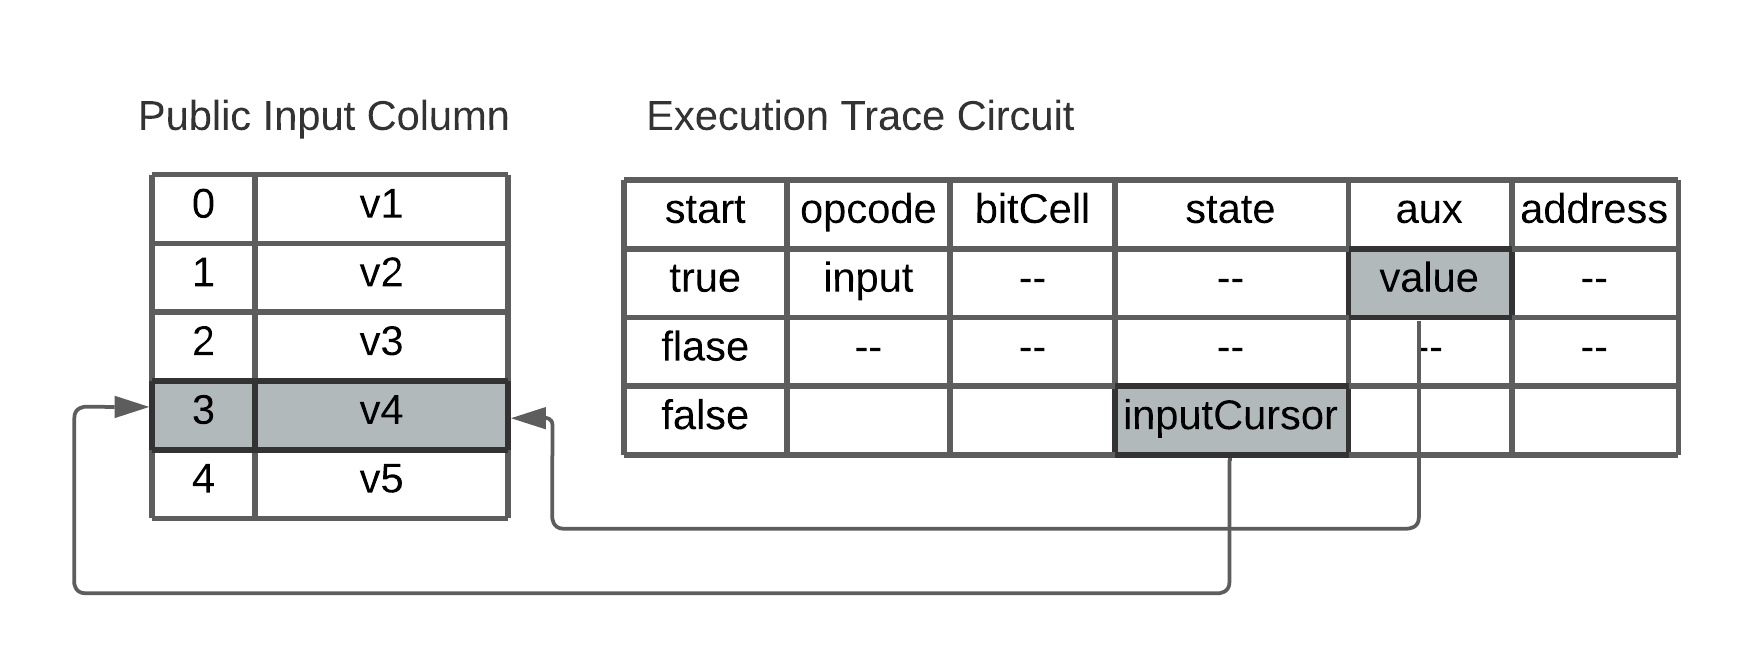
\includegraphics[scale=0.8]{figs/public-input.png}
}
\caption{Public Input Circuit}\label{fig:public-input}
\end{figure}
 Similarly we use a separate column to hold output data and use polynomial lookup to enforce that the value we output in execution circuit aux cell is the same as in the output column. When dealing with private inputs, we can put it into the stack with no constraints. (why)
\section{Instruction Circuits}
\label{chp:instruction-circuits}
Based on execution trace circuit in Section \ref{chp:architecture-circuits}, we define constraints $\mathbf{C}_{op}$ for each opcode $op$. Since the constraint defined on execution trace circuit will be applied on a row basis, and the ingredients of the constraints of each $op$ will span over multiple rows, we use notation $C(curr+k)$ to denote the $k$th cell in column $c$ followed by the current row. For example, suppose that we want to define the constraints of add instruction using the following layout (see Figure \ref{tbl:add-instruction})
\begin{table}[h]
\begin{center}
\begin{tabular}{ | c | c | c | c | c | c | c | c | c | c | c | }
  \hline
  start & opcode & bit cell & state & aux & $address \in T_{I}$ & $sp \in T_\mathcal{F}$& u64 cell & extra \\ 
  \hline
   true & $add$ & $overflow$ & $tid$ & $nil$ & $iaddr_0$ & sp & $w_0$ & $nil$\\ 
 \hline
   0 & $readStack$ & $nil$ & $nil$ & $nil$ & $nil$ & $sp_0$ & $w_1$ & $nil$\\ 
 \hline
   0 & $readStack$ & $nil$ & $nil$ & $nil$ & $nil$ & $sp_1$ & $w_2$ & $nil$\\ 
 \hline
   0 & $writeStack$ & $nil$ & $nil$ & $nil$ & $nil$ & $sp_2$ & $w_3$ & $nil$\\ 
 \hline
   true & $otherop$ & -- & $tid+1$ & $nil$ & $iaddr_1$ & $sp'$ & $w_0'$ & $nil$\\
 \hline
\end{tabular}
\caption{add circuit within execution trace circuit}
\label{tbl:add-instruction}
\end{center}
\end{table}

\noindent where $w_1$, $w_2$ are get from the stack and $w_2$ is equal to the result of the add instruction which is pushed back to the stack.
\begin{verbatim}
def add:=
    w0 = read(stack sp);
    sp0 = sp-1;
    w1 = read(stack sp0);
    w2 = (w1 + w0) mod 2^64;
    write(stack, sp0, w2);
    FALLTHROUGH
\end{verbatim}

First, we know that by definition of add opcode, $w_0 = (w_1+w_2) \bmod 2^{64}$. Thus encode the $\bmod$ semantic into arithmetic constraint, we get that $w_0 + overflow \times 2^{64}= w_1 + w_2$. Second we enforce the stack operation are valid, that are $(stack, read, sp_0, tid, 0, w0) \in T_\mathcal{M}$, $(stack, read, sp_1, tid, 1, w1) \in T_\mathcal{M}$ and $(stack, write, sp_2, tid, 2, w2) \in T_\mathcal{M}$. Third, we need to constraint that the next instruction must follow $iaddr_0$ in address, therefore $iadd_1 = iaddr_0 + 1$. In the end we constraint the $sp$ column by $sp_0 + 1= sp$, $sp_1 + 1= sp_0$, $sp_2 = sp+1$ and $sp' = sp_2$. Put it all together, and replase variables using the notation of $columnName.(curr + k)$, we have
\[
    \mathbf{C_{add}} = \begin{cases}
        &w.(curr) + bit.(curr) \times 2^{64} - w.(curr+1) + (w.curr + 2) = 0 \\
        &Plookup(T_\mathcal{M}, (stack, read, sp.(curr), tid, 0, w0)) = 0 \\
        &Plookup(T_\mathcal{M}, (stack, read, sp.(curr+1), tid, 1, w1)) = 0 \\
        &Plookup(T_\mathcal{M}, (stack, write, sp.(curr), tid, 2, w2) = 0 \\
        &iaddr.curr + 1 - iaddr.(curr + 4) = 0\\
        &sp.curr + 1 - sp.(curr+1) = 0\\
        &sp.(curr+4) - sp.(curr) - 1 = 0
    \end{cases}
\]
Since constraints are applied on a row basis of a circuit. We need to make sure that $\mathbf{C}_{add}$ does not apply on rows that is not a start row of a instruction block or a block with other opcode. So a natural way to apply $\mathcal{C}_{add}$ only on necessary rows is to multiply $\mathbf{C}_{add}(curr)$ with $curr.start \times (curr.opcode == op)$ and the final constraint related to opcode add is $\overline{\mathbf{C}}_{add}(curr) := curr.start \times (curr.opcode == op) \times \mathbf{C}_{add}(curr) = 0$.

After we constructed all the constraints $\mathcal{C}_{op_i}$ for all opcodes $op_i$, we simply sum them up and get the final constraint $\mathcal{C}_{op}(curr) := \sum_i cur.start \times (cur.opcode == op) \times \mathcal{C}_{op_i}(curr) = 0$.

\subsection{Numeric Instructions}
\label{chp:numeric-instruction}
Numeric Instructions are the majority instructions in WASM. In general, semantics of numeric instructions contains three parts, parameters preparation, arithmetic calculation, result writeback and FALLTHROUGH as follows.
\begin{verbatim}
def arithop :=
    param1 = read(stack sp); \\ parameters preparation
    param2 = read(stack (sp-1)); \\ parameters preparation
    ...
    paramN = read(stack (sp-N+1)); \\ parameters preparation
    result = arith(param1, param2, param3, ..., paramN); \\ calculation
    write(stack, (sp-N+1), result); \\ result write back
    sp = sp-N+1;
    FALLTHROUGH;
\end{verbatim}
Based on the arithmetic defintion, we assign the cells in the execution trace circuit $T_\mathcal{E}$ in Table \ref{tbl:arith-instruction}. Moreover, assume the constraint is applied on the first row of the instruction block and the constraint of arithop is defined in Equation \ref{eq:cs-arith}.
\begin{table}[!h]
\begin{center}
\begin{tabular}{ | c | c | c | c | c | c | c | c | c | c | c | }
  \hline
  start & opcode & bit cell & state & aux & $address \in T_{I}$ & $sp \in T_\mathcal{F}$& u64 cell & extra \\ 
  \hline
   true & $arithop$ & $nill$ & $tid$ & $nil$ & $iaddr_0$ & sp & $param_0$ & $nil$\\ 
 \hline
   0 & $nil$ & $nil$ & $nil$ & $nil$ & $nil$ & $nil$ & $\cdots$ & $nil$\\ 
 \hline
   0 & $nil$ & $nil$ & $nil$ & $nil$ & $nil$ & $nil$ & $param_N$ & $nil$\\ 
 \hline
   0 & $nil$ & $nil$ & $nil$ & $nil$ & $nil$ & $nil$ & $result$ & $nil$\\ 
 \hline
    true & $otherop$ & -- & $tid+1$ & $nil$ & $iaddr_1$ & $sp'$ & $w_0'$ & $nil$\\
 \hline
\end{tabular}
\caption{add circuit in execution trace circuit}
\label{tbl:arith-instruction}
\end{center}
\end{table}
\begin{equation}
    \mathbf{C_{arith}} = \begin{cases}
        &arith(param_0, param_1, ..., param_N) - result = 0 \\
        &Plookup(T_\mathcal{M}, (stack, read, sp - k, tid, k, param_k) = 0 \\
        &Plookup(T_\mathcal{M}, (stack, write, sp' - 1, tid, N, result) = 0 \\
        &iaddr_0 + 1 - iaddr_1 = 0\\
        &sp - sp' - N + 1 = 0\\
    \end{cases}
\label{eq:cs-arith}
\end{equation}
\subsection{Control Flow Instructions}
In WASM specification, there three different type of control flow: FALLTHROUGH, branch, and call (return). Implementation of the FALLTHROUGH is already covered in Section \ref{chp:numeric-instruction}. Thus it is sufficient to implement call (return) and branch.

\smallskip\noindent\emph{Call (Return) Circuit.}
Call instruction will first add a new Frame Table Entry $(tid, frameId, iaddr_0)$ into the Frame Circuits $T_\mathcal{F}$ and then loading calling parameters onto the stack and goto the $iaddr_1$ for next instruction (see Table \ref{tbl:call-instruction} for the circuit layout of \emph{call}).
\begin{table}[!h]
\begin{center}
\begin{tabular}{ | c | c | c | c | c | c | c | c | c | c | c | }
  \hline
  start & opcode & bit cell & state & aux & $address \in T_{I}$ & $sp \in T_\mathcal{F}$& u64 cell & extra \\ 
  \hline
   true & $call(targetIaddr)$ & $nill$ & $tid$ & $nil$ & $iaddr_0$ & sp & $param_0$ & $nil$\\ 
 \hline
   0 & $nil$ & $nil$ & $pFrameId$ & $nil$ & $nil$ & $nil$ & $\cdots$ & $nil$\\ 
 \hline
   0 & $nil$ & $nil$ & $nil$ & $nil$ & $nil$ & $nil$ & $param_N$ & $nil$\\ 
 \hline
   true & $otherop$ & -- & $tid + 1$ & $nil$ & $iaddr_1$ & $sp'$ & $nil$ & $nil$\\
 \hline
   0 & $nil$ & $nil$ & $nFrameId$ & $nil$ & $nil$ & $nil$ & $nil$ & $nil$\\ 
 \hline
\end{tabular}
\caption{circuit layout of call}
\label{tbl:call-instruction}
\end{center}
\end{table}

\noindent where the circuit constraint is:
\[
    C_{call} = \begin{cases}
        &Plookup(T_\mathcal{M}, (stack, write, sp+i, tid, i, param_i)) = 0 \\
        &Plookup(T_\mathcal{F}, (tid, pFrameId, iaddr_0)) = 0 \\
        &iaddr_1 - targetIaddr = 0\\
        &sp' - sp - N = 0 \\
        &nFrameId - tid = 0
    \end{cases}
\]

 As we mentioned in Section \ref{chp:frame-circuit}, all the entries in $T_\mathcal{F}$ is used to help the return instruction to find the correct calling frame so that we can define the semantic of \emph{return} by finding the correct return \emph{iaddr} in $T_\mathcal{F}$ (see Table \ref{tbl:return-instruction} for the circuit layout of \emph{return}).
\begin{table}[!h]
\begin{center}
\begin{tabular}{ | c | c | c | c | c | c | c | c | c | c | c | }
  \hline
  start & opcode & bit cell & state & aux & $address \in T_{I}$ & $sp \in T_\mathcal{F}$& u64 cell & extra \\ 
  \hline
   true & $return$ & $nill$ & $tid$ & $nil$ & $iaddr_0$ & sp & $nil$ & $nil$\\ 
 \hline
   0 & $nil$ & $nil$ & $prevFrameId$ & $nil$ & $nil$ & $nil$ & $nil$ & $nil$\\ 
 \hline
   true & $otherop$ & -- & $tid + 1$ & $nil$ & $iaddr_1$ & $sp'$ & $nil$ & $nil$\\
 \hline
   0 & $nil$ & $nil$ & $nFrameId$ & $nil$ & $nil$ & $nil$ & $nil$ & $nil$\\ 
 \hline
\end{tabular}
\caption{circuit layout of return}
\label{tbl:return-instruction}
\end{center}
\end{table}
and the circuit constraint is Equation \ref{eq: cs-return}.
\begin{equation}
    C_{return} =  \begin{cases}
        &Plookup(T_\mathcal{F}, (pFrameId, nFrameId iaddr_1 - 1)) = 0 \\
        &sp' - sp = 0 \\
    \end{cases}
\label{eq: cs-return}
\end{equation}

\smallskip\noindent\emph{Branch Circuit.}
Branch instructions in WASM includes \emph{br}, \emph{br\_if}, \emph{if * then * else *}, etc. The semantics of branch instructions can be uniformly abstract as three steps. First, read related parameters from the stack. Seconde, calculate the target branch address according to the params. Third, branch to the target branch address.
\begin{verbatim}
def branchop :=
    param1 = read(stack sp); \\ parameters preparation
    param2 = read(stack (sp-1)); \\ parameters preparation
    ...
    paramN = read(stack (sp-N+1)); \\ parameters preparation
    iaddr1 = select(param1, param2, ..., paramN); \\ calculate branch address
    GOTO iaddr2;
\end{verbatim}
\smallskip The circuit layout of branch instruction is sketched in Table \ref{tbl:branch-instruction} and its circuit constraint is defined in Equation \ref{eq:cs-branchop}. 
\begin{table}[!h]
\begin{center}
\begin{tabular}{ | c | c | c | c | c | c | c | c | c | c | c | }
  \hline
  start & opcode & bit cell & state & aux & $address \in T_{I}$ & $sp \in T_\mathcal{F}$& u64 cell & extra \\ 
  \hline
   true & $branchop$ & $nill$ & $tid$ & $nil$ & $iaddr_0$ & sp & $param_0$ & $nil$\\ 
 \hline
   0 & $nil$ & $nil$ & $pFrameId$ & $nil$ & $nil$ & $nil$ & $\cdots$ & $nil$\\ 
 \hline
   0 & $nil$ & $nil$ & $nil$ & $nil$ & $nil$ & $nil$ & $param_N$ & $nil$\\ 
 \hline
   true & $otherop$ & -- & $tid + 1$ & $nil$ & $iaddr_1$ & $sp'$ & $nil$ & $nil$\\
 \hline
   0 & $nil$ & $nil$ & $nFrameId$ & $nil$ & $nil$ & $nil$ & $nil$ & $nil$\\ 
 \hline
\end{tabular}
\caption{circuit layout of call}
\label{tbl:branch-instruction}
\end{center}
\end{table}
\begin{equation}
    C_{call} = \begin{cases}
        &Plookup(T_\mathcal{M}, (stack, write, sp+i, tid, i, param_i)) = 0 \\
        &iaddr_1 - select(param_0, param_1, \cdots) = 0 \\
        &nFrameId - pFrameId = 0
    \end{cases}
\label{eq:cs-branchop}
\end{equation}

\subsection{Memory (Stack, Global) Instructions}
Memory, Stack and Global instructions can be abstract as a tuple of \emph{(category=Memory|Stack|Global, type=INIT|READ|WRITE, address, size = 8|16|32|64, value)} and the layout of the circuit is defined Table \ref{tbl:memory-instruction}. By using the access log circuit defined in Chapter \ref{chp:access-log-circuit}, the constraint for memory circuit is simply $(category, ltype, tid, address, value') \in T_\mathcal{M} \wedge trunc(value', size) = value$.

\begin{remark}
For read, this constraint ensures the result read from $address$ is valid. For write, $T_\mathcal{M}$ ensures that the next $read$ of $address$ will return the previous written value correctly.
\end{remark}
\begin{table}[!h]
\begin{center}
\begin{tabular}{ | c | c | c | c | c | c | c | c | c | c | c | }
  \hline
  start & opcode & bit cell & state & aux & $address \in T_{I}$ & $sp \in T_\mathcal{F}$& u64 cell & extra \\ 
  \hline
   true & $op(type, size)$ & $nill$ & $tid$ & $nil$ & $iaddr_0$ & sp & $address$ & $nil$\\ 
 \hline
   0 & $nil$ & $nil$ & $frameId$ & $nil$ & $nil$ & $nil$ & $value$ & $nil$\\ 
 \hline
   true & $otherop$ & -- & $tid + 1$ & $nil$ & $iaddr_1$ & $sp'$ & $w_0'$ & $nil$\\
 \hline
   0 & $nil$ & $nil$ & $frameId = tid$ & $nil$ & $nil$ & $nil$ & $w_3$ & $nil$\\ 
 \hline
\end{tabular}
\caption{memory access circuit within execution trace circuit}
\label{tbl:memory-instruction}
\end{center}
\end{table}

\section{Customized Instruction Extension}
\label{chp:foreign}
Just like architecture specific instructions in normal hardware, \zkwasm\, supports customizing foreign instruction extension as well. More specificly, \zkwasm\, provides two ways to extend the instructions set, one way is implementing customized inline opcodes and the other way is batching external proofs of pure functions.

Given a fixed image, an entry function and an array of input arguments, the execution trace is fixed which means the number of instructions are fixed. As we described in Section \ref{chp:ex-table}, each instruction occupies $n$ (a fixed number of) rows in the execution circuit $T_\mathcal{E}$. Thus the total rows of $T_\mathcal{E}$ is fixed. When doing proof in Halo2 using KZG commitment, each column is interpolated into polynomials using FFT (fast fourier transform). Because FFT is an algorithm of $NlogN$ complexity, the total rows of $T_\mathcal{E}$ affacts the overall performance in a nonlinear way. Thus to reduce the number of columns, a good way is to batch multiple instructions into one.

When the semantic of instructions we would like to batch is simple and can fit into one instruction block, we can use the inline extension. For example, suppose that we want to sum the lowest 4 bits $x:u64$ by function $sumLowest(x)$. If we use a standard loop to implement the algorithm, it will takes $4$ instructions to extract $4$ bits and takes another $2$ to do the sum. However, if we inline this function in to a foreign function, then we can encode the arithmetic constraint within one instruction block. As a case study, we compare the SHA256 execution trace with and without inline the following macro:

\begin{table}[!h]
\small
\begin{center}
\begin{tabular}{ | c | p{1cm} | c | p{1.5cm} | }
  \hline
  original & original rows & customized & optimized rows\\ 
  \hline
  $\lambda x, y, (x \& y) | (complete(x) \& z)$ & 4 & $ch(x,y)$ & 1 \\
  \hline
  $\lambda x, y, z, z | (x \& (y | z))$ & 2 & $maj(x, y, z)$ & 1\\
  \hline
  $\lambda x, rotr_{32}(x, 2) | rotr_{32}(x, 13) | rotr_{32}(x, 22)$ & 5 & $lsigma0(x)$ & 1 \\
  \hline
  $\lambda x, rotr_{32}(x, 6) | rotr_{32}(x, 11) | rotr_{32}(x, 25)$ & 5 & $lsigma1(x)$ & 1\\
 \hline
   sha256 using pure WASM instructions & 1 & sha256 using customized instructions & XXX\\
 \hline
\end{tabular}
\caption{row reduce by using customized instructions}
\label{tbl:memory-instruction}
\end{center}
\end{table}


\section{Program partition and proof batching}
\label{chp:sharding-batching}
As discussed in Section \ref{chp:foreign}, when encoding execution trace in $T_\mathcal{E}$, each instruction will take a constant number of rows. In Halo2 proof system, there is a limit to the total number of rows of arithmetic circuits \cite{halo2book}. Therefore, for large WASM images, we probably can not fit the whole execution trace into $T_\mathcal{E}$. To solve the problem of long execution trace,  \zkwasm\, use the technique of program partition and proof batching. The idea is that we split the execution trace $\left[t_0,t_1,\cdots\right]$ into a group of sub sequences, generate execution proof for each group and batch all the proofs in the end. Here we first give a bold sketch of the overview of the technique and then presents the extra constraints we need to provide when batching sub proofs.

\smallskip Given an execution sequence $t_i$, we split it into small execution chunks $t_{[a,b]} = {t_a, t_{a+1}, \cdots, t_{b-1}}$ and denote the $\mathcal{M}_{[a,b]}, \mathcal{SP}_{[a,b]}$, $\mathcal{G}_{[a,b]}$ to be the memory, stack and global access log related to $t_{[a,b]}$. We notice that given an execution trace $t_{[a,b]}$, by using the arithmetic circuits constructed in Section \ref{chp:architecture-circuits}, we can prove $t_{[a,b]}$ is valid under the context \partialstate{a}{b}. We denote $\mathcal{P}_{[a,b]}$ the proof of the valid execution of $t_{[a,b]}$ and $\mathcal{P}$ is the proof of the valid execution of $t_i$ under the full access log \fullstate. Now it remains to find out what conditions we need to enforce so that
\[
   (\mathcal{P}_{[0,k-1]} \wedge   \mathcal{P}_{[k,2k-1]} \wedge \cdots \wedge   \mathcal{P}_{[0,end]}) \rightarrow
     \mathcal{P}.
\]
\noindent Thus it is sufficient to make sure that for each $t_i \in t_{[a,b]}$ the constraints applied on it in $\mathcal{P}_{[a,b]}$ is equivalent to the constraints applied on it in $\mathcal{P}$. As we have presented in Section \ref{chp:architecture-circuits}, constraints applied on each instruction block in $T_\mathcal{E}$ contains two parts, that are polynomial constraints about cells of the current and next instruction block and constraints of polynomial lookup of state (memory, stack, global) access logs.\\

\noindent\emph{Equivalent of Polynomial Constraints.} Regarding the polynomial constraints of cells, it is easy to check that if $t_i\in t_{[a,b]}$ and $i<b$ then all polynomial constraints of cells of the instruction block of $t_i$ in $\mathcal{P}_{[a,b]}$ are equal to the those in $\mathcal{P}$. So it remains to constrain that the last instruction of $t_{[a,b]}$ has the same polynomial constraints both in $\mathcal{P}_{[a,b]}$ and $\mathcal{P}$. However, it is not true in general since if we split the execution sequence into blocks that are disjoint, then the connection between the two sequences is lost. Therefore, to solve this problem, we need to pad a glue instruction at the end of each sub sequence and enforce the address of the glue instruction equal to the address of the first instruction of the next block (see Figure \ref{fig:subsequence}). By doing so we can check that the polynomial constraints of each $t_i$ in $\mathcal{P}_{[a,b]}$ is equivalent as it is in $\mathcal{P}$. \\

\begin{figure}[!ht]
\centerline{
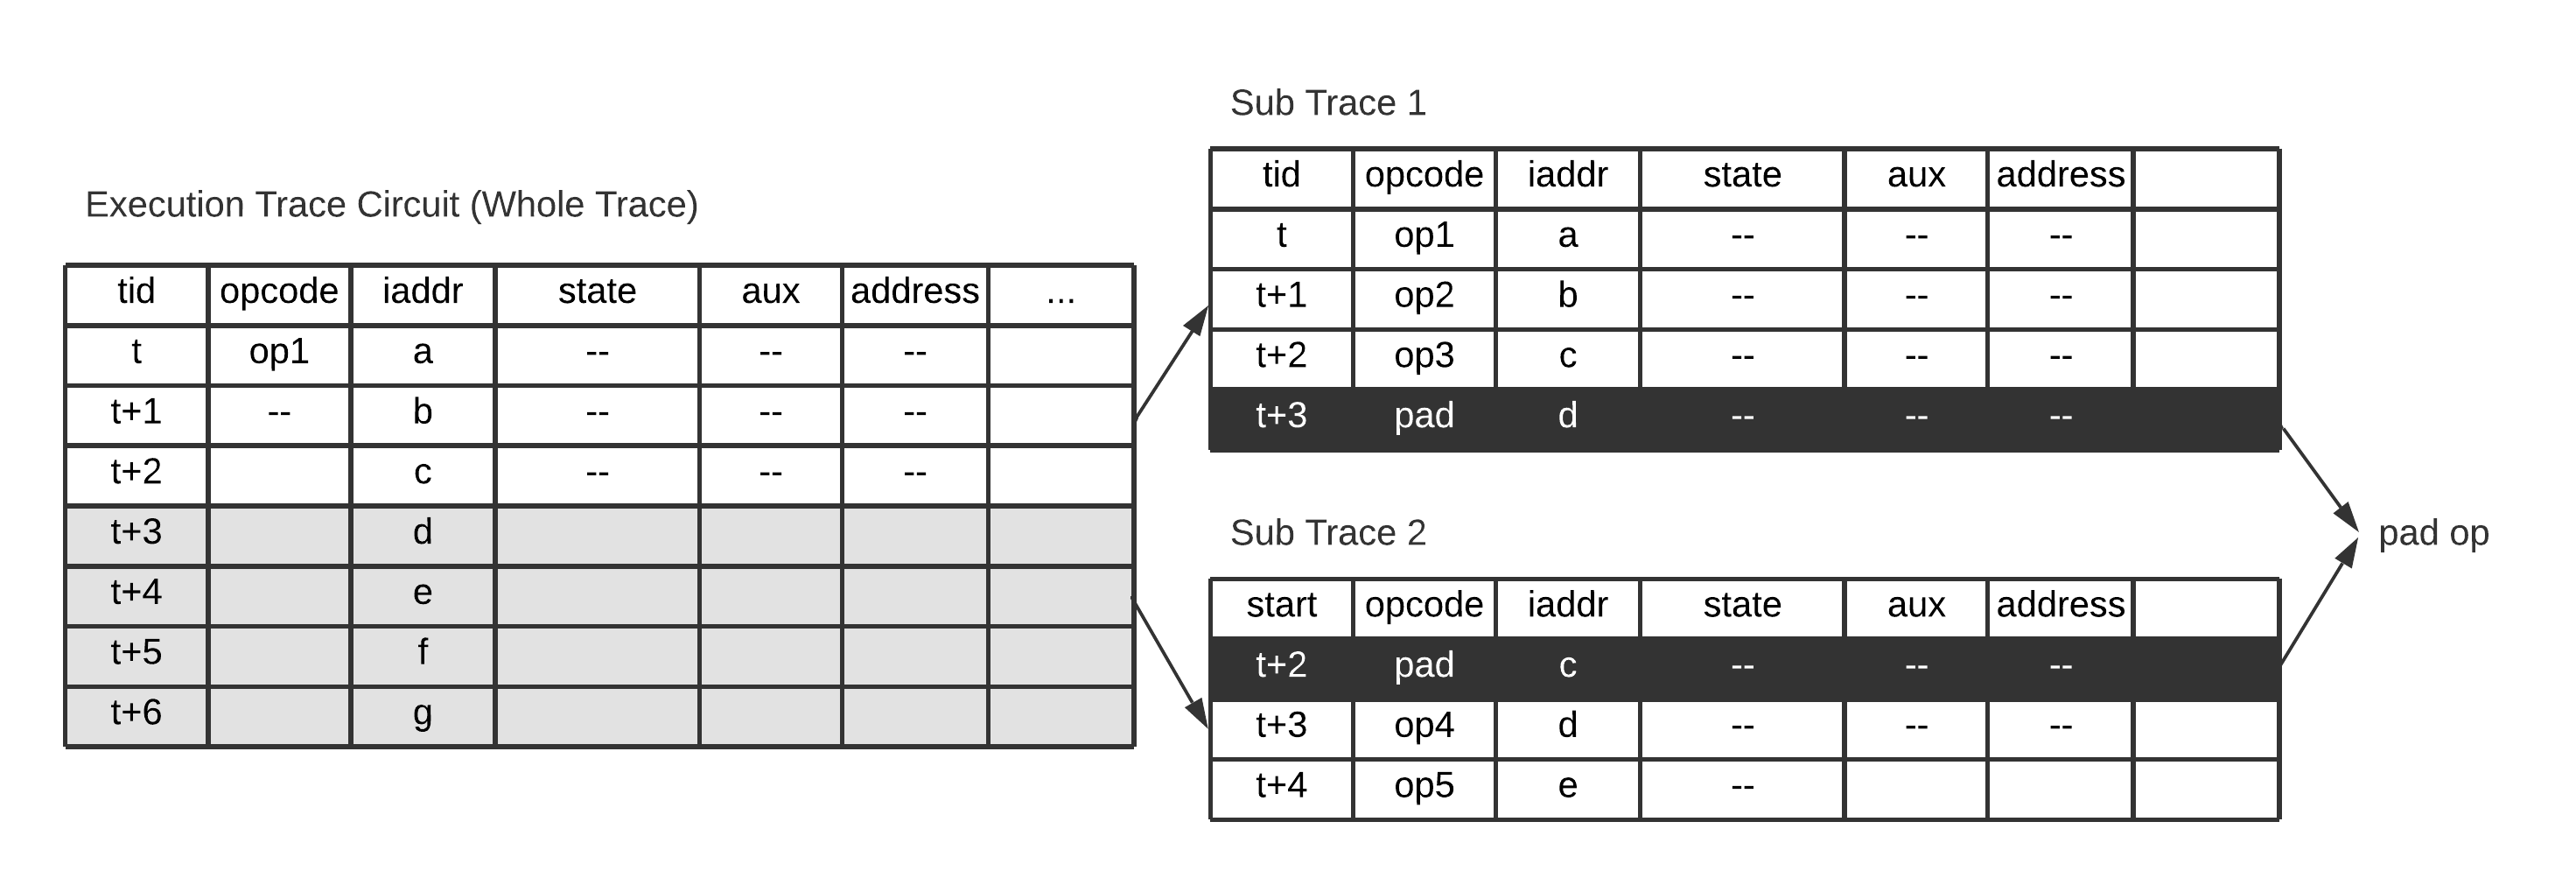
\includegraphics[scale=0.6]{figs/subsequence.png}
}
\caption{Split execution sequence into sub sequence}
\label{fig:subsequence}
\end{figure}

\noindent\emph{Equivalent of Polynomial Lookup.} Given a constraint of polynomial lookup for a cell in $t_i$, we need to show that $c \in \mathbf{T}_\mathcal{M}$ if and only if $c \in \cup \mathbf{T}_{\mathcal{M}_{k}}$. By the definition of Equation \ref{eq:rw-constraints} we know that the property hold if and only if the concatenate of $\mathbf{T}_{\mathcal{M}_k}$ satisfies Equation \ref{eq:rw-constraints}. Notice that Equation \ref{eq:rw-constraints} only constraints adjacent rows, we extract a glue table $\mathbf{TG}_\mathcal{M}$ for $\mathbf{T}_{\mathcal{M}_{k}}$ ($k = 1,2,\cdots$) as in (Figure \ref{fig:tbl-glue}) and then it follows that $\mathbf{T}_\mathcal{M} = \cup \mathbf{T}_{\mathcal{M}_{k}}$ if $\mathbf{T}_\mathcal{M}$, $\mathbf{T}_{\mathcal{M}_{k}}$ and $\mathbf{TG}_\mathcal{M}$ all satisfy Equation \ref{eq:rw-constraints}.

\begin{figure}[!ht]
\centerline{
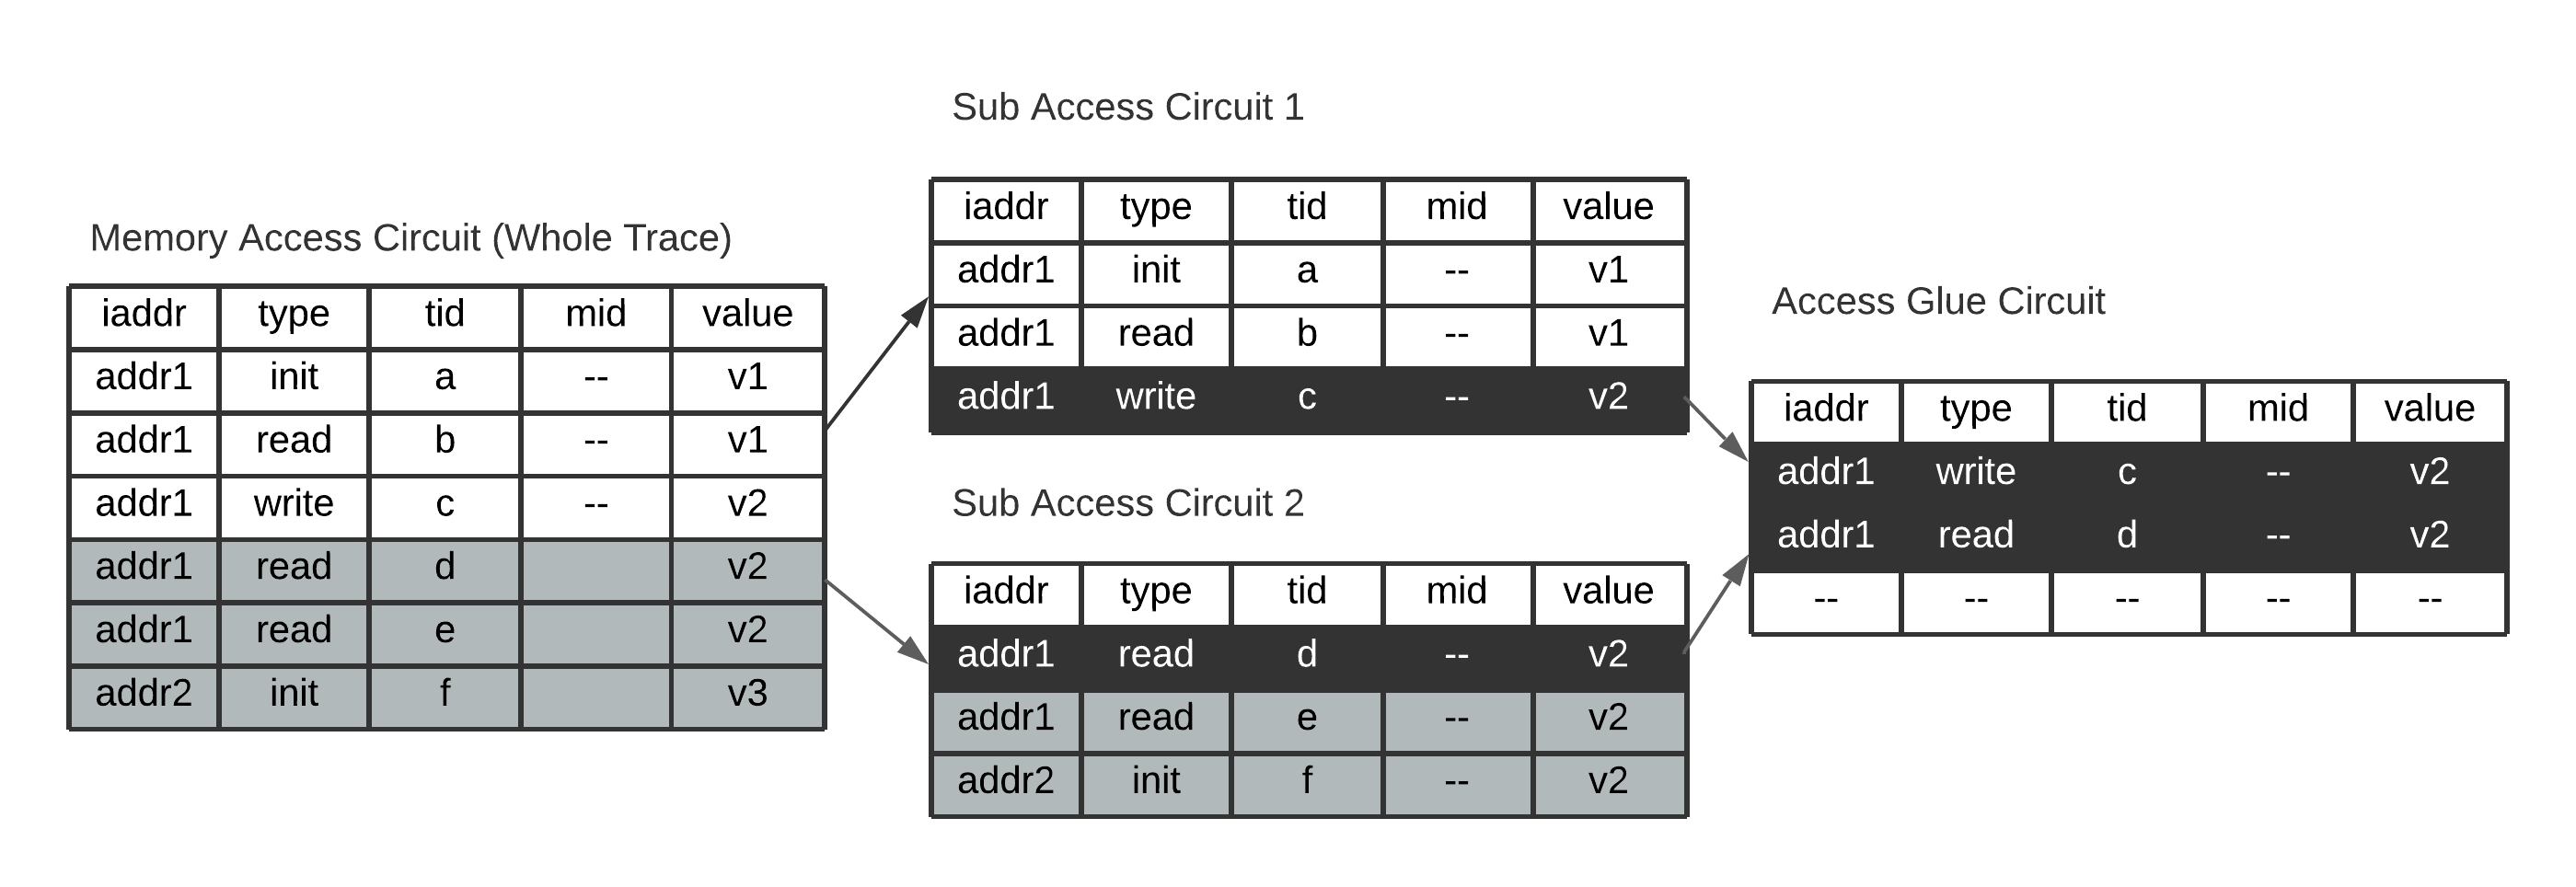
\includegraphics[scale=0.6]{figs/memory-glue.png}
}
\caption{Split memory access log into sub log}
\label{fig:tbl-glue}
\end{figure}

\smallskip As a conclusion, to solve the long execution trace problem, we split the execution trace into $t_{[a_0,b_0]}, t_{[a_1,b_1]}, t_{[a_2, b_2]}, \cdots$ and construct $\mathbf{T}_{\mathcal{M}_{k}}$ $\mathbf{T}_{\mathcal{SP}_{k}}$ $\mathbf{T}_{\mathcal{G}_{k}}$ for execution block $t_{[a_k, b_k]}$. Suppose that $\mathcal{P}_k$ proves the valid execution of $t_{[a_k,b_k]}$ and $\mathbf{TG}_\mathcal{M}$ is the gluing map constructed as in Figure \ref{fig:tbl-glue}, then we claim that a proof $\mathcal{P}_{batch}$ can prove that the execution sequence $t_i$ is a valid execution if and only if $\mathcal{P}_{batch}$ is the batched proof of all the constraints in Equation \ref{eq:split-eq}.
\begin{equation}
   \begin{cases}
        \mathcal{P}_k \textrm{ proves }  t_{[a_k,b_k]} \textrm{ is a valid execution under } (\mathcal{F}, \mathcal{M}_{[a_k,b_k]}, \mathcal{SP}_{[a_k,b_k]}, \mathcal{I}(\mathcal{C,\mathcal{H}})). \\
        t_{b_{k+1}}.iaddr = t_{a_{k}}.iadr \textrm{ when $k>0$ }. \\
        t_{b_{k}} \textrm{ is a glue instruction when $k>0$ and $t_{[a_k, b_k]}$ is not the last exectuion block}. \\
        TG_\mathcal{M} \textrm { satisfies Constraint \ref{eq:rw-constraints}}. \\
   \end{cases}
    \label{eq:split-eq}
\end{equation}

\noindent In \zkwasm, we write the verifying algorithm of $\mathcal{P}_k$ into arithmetic circuits $\mathcal{V}_k$ and the total batch circuit of Equation \ref{eq:split-eq} is construct by putting the verifying circuits together with the circuits that do the other simple checks.

\begin{remark}
Proof batching is an active research topic. Instead of writing verify function into arithmetic circuits, there are other methods \cite{ben2017scalable-batch,chiesa2019cycles-batch,habock2021darlin-batch,kothapalli2022nova-batch} that are worth trying as well. Since we focus more on the consistency of program partition and memory access log in this paper, we leave the analysis of trying different batching methods as future work.
\end{remark}
\section{Performance Benchmark}
\label{chp:performance}
All the benchmark test suites are run on a machine with AMD Ryzen 7 5800X3D 8-Core Processor, one GeForce RTX 3090 graphic card and 32G * 4 DDR4 2133 ram.

\subsection{Performance without Program Partition and Proof Batching}
Among programs whose valid execution trace fits into the max sequence size of \zkwasm, we measure the performance of \zkwasm\, when dealing with two special programs: the Fibonacci function which has a deep call stack and the binary search function which has frequent memory access. As shown in Table \ref{tbl:fib} and Table \ref{tbl:bsearch}, circuit size $CS$ denotes the total number of rows of circuits in \zkwasm, as a power of $2$ and trace size denotes the total instructions included in the execution trace. Proof time is the time \zkwasm used to create the proof for the valid execution and the verify time is the time for a verifier to check the proof. The column \emph{memory swap} indicates whether the overall memory consumption is large than 128G.
\begin{table}[!h]
\small
\begin{center}
\caption{Benchmark for fibonacci in \zkwasm}
\label{tbl:fib}
\begin{tabular}{ | c | c | c | c | c| c| }
  \hline
  circuit size & trace size & call depth & proof time & verify time & memory swap\\ 
  \hline
  18 & 9037 & 13 & 44s & 22 ms & false\\
  \hline
    19 & 23677 & 15 & 88s & 24 ms & false \\
  \hline
    20 & 38317 & 16 & 178s & 22 ms & false \\
  \hline
    21 & 100333 & 18 & 358s & 22ms & false\\
  \hline
    22 & 162349 & 19 & 828s & 29ms & true \\
  \hline
\end{tabular}

\end{center}
\end{table}

\begin{table}[!h]
\small
\begin{center}
\caption{Benchmark for binary search in \zkwasm}
\label{tbl:bsearch}
\begin{tabular}{ | c | c | c | c | c | c | }
  \hline
  circuit size & trace size & search buf size (64k per page) & proof time & verify time & memory swap\\ 
  \hline
  18 & 585 & 26 & 44.200s & 22 ms & false\\
  \hline
    19 & 616 & 63 & 87.200s & 24 ms & false \\
  \hline
    20 & 647 & 124 & 173.200s & 22 ms & false \\
  \hline
    21 & 678 & 246 & 342.200s & 24ms & false\\
  \hline
    22 & 809 & 490 & 803.200s & 25ms & true \\
  \hline
\end{tabular}

\end{center}
\end{table}

From Table \ref{tbl:fib} and Table \ref{tbl:bsearch} we see that the verifying time is O(1) and proof time grows linearly when the size of the circuit grows. When the memory usage is small, the instruction volume grows linearly as the circuit size grows (see Table \ref{tbl:fib}). When the memory consumption grows linearly as the circuit size grows, the instruction volume grows slowly as shown in Table \ref{tbl:bsearch}.


\subsection{Performance for Large Program with Proof Batching}
For a program with a large execution sequence, we split the execution trace into partitions and generate a sub-proof for each partition. To batch these sub proofs, we use the batching circuit (see Section \ref{chp:sharding-batching}) to generate a batched proof. Therefore the time of creating a final proof of a large program is the sum of sub-proof generation time plus the proof batching time.
\begin{table}[!h]
\small
\begin{center}
\caption{Benchmark for proof batching in \zkwasm}
\label{tbl:proof-batching}
\begin{tabular}{ | c | c | c | c | c | c | c| }
  \hline
  partition CS & partition proof & total pieces& batching CS & batching proof & verify time & memory swap\\ 
  \hline
  18 & 2 & 1 & 22 & 168s & 4.7 ms & false\\
  \hline
  18 & 2 & 2 & 22 & 326s & 4.63 ms & false\\
  \hline
    20 & 2 & 1 & 22 & 168s & 4.77 ms & false \\
  \hline
    20 & 2 & 2 & 22 & 324s & 5.05ms & false\\
  \hline
    22 & 2 & 1 & 22 & 168s & 5.07ms & false\\
  \hline
    22 & 2 & 2 & 22 & 325s & 4.93ms & true \\
  \hline
\end{tabular}
\end{center}
\end{table}
It can be seen in Table \ref{tbl:proof-batching} that the proving time for batching sub-proofs with different partition size is constant and the only factor that affects the batching proof time is the number of pieces of sub-proof. 

In conclusion, if we have a large program for \zkwasm\, and we want to optimize the total time of generating the final proof, then the factors we need to consider are the following: First, What is the partition size we use to split the whole transaction sequence. Second, how many pieces we should put together in one proof batch. Third, how we generate the proofs in parallel.

\section{Conclusion \& Further Work}
\label{chp:conclusion}
We presented \zkwasm, a WASM virtual machine that leverages the technology of \zksnark. As far as know, we are the first to present a novel way to implement the semantics of a WASM virtual machine in arithmetic circuits. Using \zkwasm, we will be able to deploy serverless service in an untrusted cloud since \zkwasm\, does not only emulates the execution but also gives a correctness proof of the execution result. Thus any vulnerability on the cloud will not affect the correctness of the verifiable result (a faulty result can not have correct ZKSNARK proof).

For large applications that provide large execution traces, we successfully applied the execution partition and proof batching technique so the \zkwasm\, scales when the program size grows. Regarding the performance, various optimization can be applied in the future including improving the commitment scheme \cite{chen2022hyperplonk}, adopting a better parallel computing strategy \cite{wu2018dizk}, using SNARK specific hardware \cite{peng2020design, xavier2022pipemsm}, etc.




\bibliographystyle{plain}
\bibliography{main}

\end{document}
\endinput
%%
%% End of file `sample-acmsmall.tex'.
